\chapter{Sistemas Magnéticos Nanoscópicos} % Main chapter title

\label{Chapter3}% Change X to a consecutive number; for referencing this chapter elsewhere, use \ref{ChapterX}

\definecolor{mygreen}{rgb}{0,0.6,0}
\definecolor{mygray}{rgb}{0.5,0.5,0.5}
\definecolor{mymauve}{rgb}{0.58,0,0.82}

%%%%%%%%%%%%%%%%%%%%%%%%%%%%%%%%%%%%%%%%%%%%%%%%%%%%%%%%%%%%%%%%%%%%%%%%%%%%%
% parámetros para configurar el formato del código en los entornos lstlisting
%%%%%%%%%%%%%%%%%%%%%%%%%%%%%%%%%%%%%%%%%%%%%%%%%%%%%%%%%%%%%%%%%%%%%%%%%%%%%
\lstset{ %
  backgroundcolor=\color{white},   % choose the background color; you must add \usepackage{color} or \usepackage{xcolor}
  basicstyle=\footnotesize,        % the size of the fonts that are used for the code
  breakatwhitespace=false,         % sets if automatic breaks should only happen at whitespace
  breaklines=true,                 % sets automatic line breaking
  captionpos=b,                    % sets the caption-position to bottom
  commentstyle=\color{mygreen},    % comment style
  deletekeywords={...},            % if you want to delete keywords from the given language
  %escapeinside={\%*}{*)},          % if you want to add LaTeX within your code
  %extendedchars=true,              % lets you use non-ASCII characters; for 8-bits encodings only, does not work with UTF-8
  %frame=single,	                % adds a frame around the code
  keepspaces=true,                 % keeps spaces in text, useful for keeping indentation of code (possibly needs columns=flexible)
  keywordstyle=\color{blue},       % keyword style
  language=[ANSI]C,                % the language of the code
  %otherkeywords={*,...},           % if you want to add more keywords to the set
  numbers=left,                    % where to put the line-numbers; possible values are (none, left, right)
  numbersep=5pt,                   % how far the line-numbers are from the code
  numberstyle=\tiny\color{mygray}, % the style that is used for the line-numbers
  rulecolor=\color{black},         % if not set, the frame-color may be changed on line-breaks within not-black text (e.g. comments (green here))
  showspaces=false,                % show spaces everywhere adding particular underscores; it overrides 'showstringspaces'
  showstringspaces=false,          % underline spaces within strings only
  showtabs=false,                  % show tabs within strings adding particular underscores
  stepnumber=1,                    % the step between two line-numbers. If it's 1, each line will be numbered
  stringstyle=\color{mymauve},     % string literal style
  tabsize=2,	                   % sets default tabsize to 2 spaces
  title=\lstname,                  % show the filename of files included with \lstinputlisting; also try caption instead of title
  morecomment=[s]{/*}{*/}
}





\begin{figure}[H]
  \begin{minipage}[b]{0.47\textwidth}
     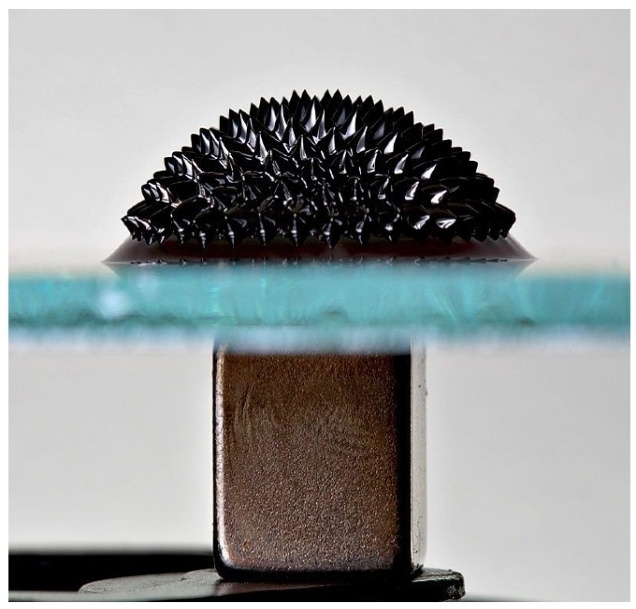
\includegraphics[width=1.10\textwidth]{./Figures/fig30}
  \end{minipage}
  \hfill
  \begin{minipage}[b]{0.47\textwidth}
     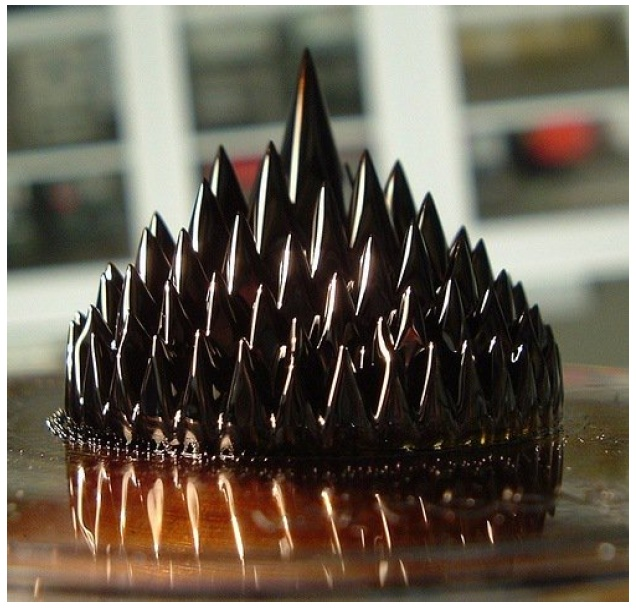
\includegraphics[width=1.10\textwidth]{./Figures/fig31}
  \end{minipage}
	\caption{Ferrofluidos en campos magnéticos}
	\label{fig:30}
\end{figure}

\vspace{10mm}

\begin{center}
Caminábamos en\\
direcciones opuestas\\
Hasta encontrarnos cada vez\\
Más juntos\\
Atraídos por el magnetismo\\
de nuestras\\
Incompatibilidades

\hspace{4.0cm} Magnetismo\\
\hspace{3.2cm} Rubén Sampietro  
\end{center}

\begin{figure}[H]
    \centering
    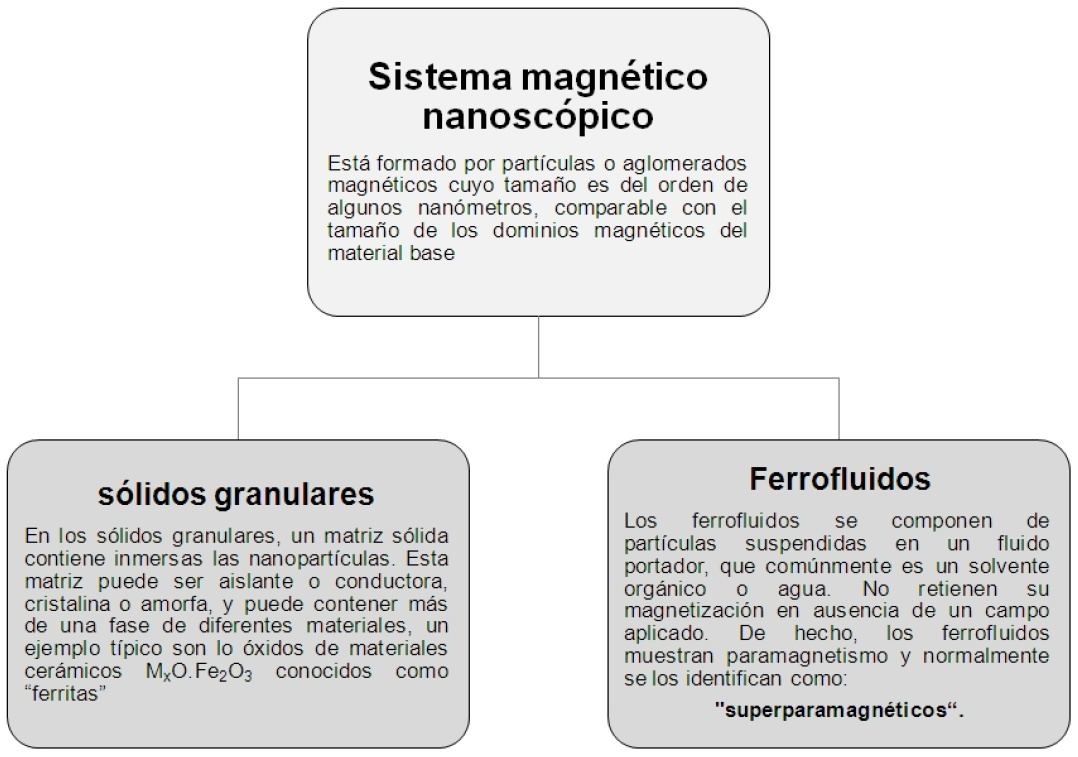
\includegraphics[width=1.19\textwidth]{./Figures/fig32}
\end{figure}


\section{Superparamagnetismo}

$\centerdot$ Una propiedad notable de los materiales ferromagnéticos y ferrimagnéticos no es tanto que tengan una magnetización espontánea, sino que su magnetización puede verse influenciada por la aplicación de campos magnéticos muy bajos. Incluso el campo de la tierra ($20-50 \mu T$) puede causar cambios de magnetización a pesar de que las fuerzas de intercambio interatómicas responsables de la magnetización espontánea son equivalentes a un campo de aproximadamente $1000 T$, casi 100 millones de veces más que el campo de la tierra. Lo que permite que esto ocurra es el hecho de que la muestra está compuesta de pequeñas regiones, que son los dominios magnéticos, dentro de cada una de las cuales la magnetización local está saturada pero no necesariamente paralela. Los dominios son pequeños ($1-100 \mu m$), pero mucho más grandes que las distancias atómicas. Este fenómeno se pone de manifiesto en el superpamagnetismo.

$\centerdot$ El Superparamagnetismo es un tipo de magnetismo que ocurre en materiales ferromagnéticos o ferrimagnéticos, cuando estos están formados por partículas muy pequeñas, de escala nanométrica (rango de 1-100 nm). Dependiendo del material, estas nanopartículas poseen dominio magnético simple o mono dominio. En estos casos se hace comparable el tamaño de la partícula con el dominio. Estas nanopartículas se magnetización en la dirección de fácil magnetización. Es importante destacar que cualquier partícula mono dominio se encuentra en un estado de magnetización uniforme en cualquier campo magnético, este comportamiento de la magnetización es idéntico al paramagnetismo frente a un campo externo. La diferencia es que el momento magnético de las nano partículas es mucho mayor, a este fenómeno con momentos magnéticos grandes aún en presencia de campos pequeños, se lo conoce como Superparamagnetismo

$\centerdot$ Los materiales superparamagnéticos tienen una alta magnetización de saturación y nula coercitividad y remanencia, por lo que se distingue de los ferromagnéticos y paramagnéticos, no hay área bajo el ciclo de histéresis, como se muestra en la gráfica de la figura \ref{fig:33}.

\begin{figure}[H]
    \centering
    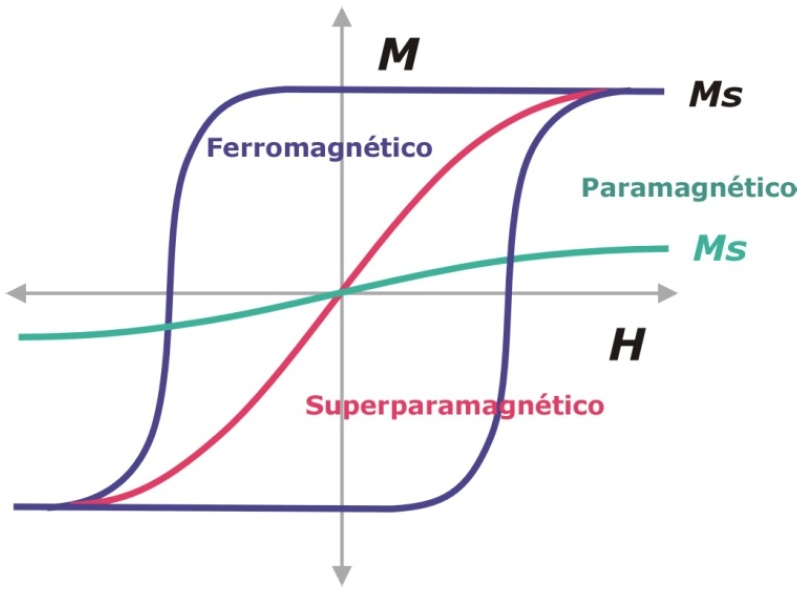
\includegraphics[width=0.6\textwidth]{./Figures/fig33}
	\caption{Ferro, Para y Superpara magnéticos}
	\label{fig:33}    
\end{figure}

$\centerdot$ El superparamagnetismo es un efecto de tamaño del material ferromagnético. Como se ve en el esquema inferior, que muestra la influencia del tamaño de partícula magnético sobre las propiedades magnéticas. La coercitividad cambia con el tamaño de partícula y, a un tamaño lo suficientemente pequeño, la coercitividad se vuelve cero.

En el gráfico de la figura \ref{fig:34} se observa el comportamiento cualitativo de la coercitividad de las partículas magnéticas en función del tamaño. El comportamiento magnético de las nanopartículas superparamagnéticas se demuestra mediante la línea roja, mientras que las partículas ferromagnéticas (FM) se presentan mediante líneas verdes y azules.


\begin{figure}[H]
    \centering
    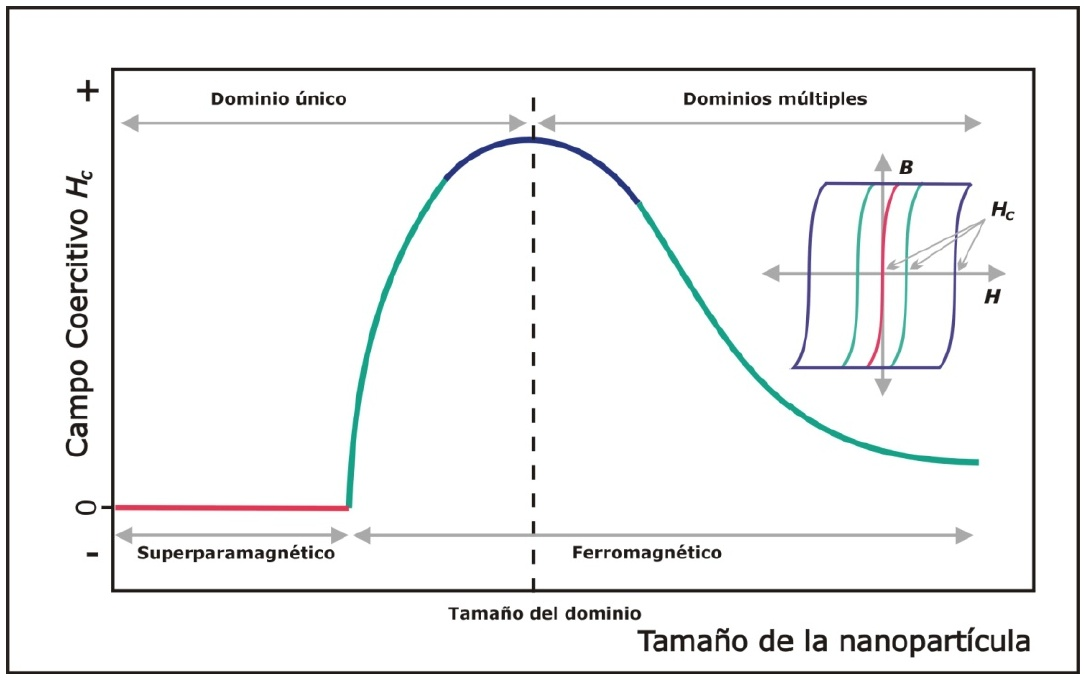
\includegraphics[width=0.9\textwidth]{./Figures/fig34}
	\caption{Comportamiento cualitativo}
	\label{fig:34}    
\end{figure}

$\centerdot$ El superparamagnetismo ocurre en partículas con tamaños más pequeños que el límite superparamagnético, este límite es menor que el tamaño medio de dominio tal como se ve en la figura \ref{fig:35}. Observemos que este fenómeno se da por debajo de la temperatura de Curie, sin embargo el material continúa manteniendo una alta susceptibilidad magnética como en el caso ferromagnético.

\begin{figure}[H]
    \centering
    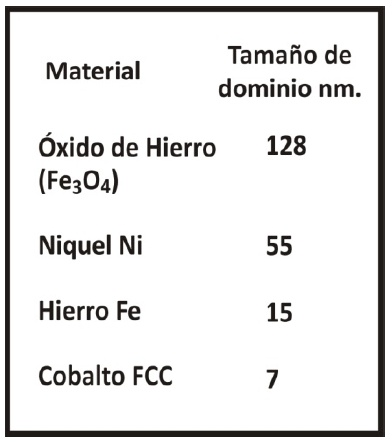
\includegraphics[width=0.5\textwidth]{./Figures/fig35}
	\caption{Comportamiento cualitativo}
	\label{fig:35}    
\end{figure}

$\centerdot$ En 1959, Bean y Livingston plantean que el momento magnético en el interior de cada partícula se lo puede pensar como $\mu=N\mu_{at}$.donde $N$ es el número de átomos magnéticos en la partícula y $\mu_{at}$ es el momento magnético atómico. Una vez que se retira el campo magnético exterior la magnetización describe una ley tipo Arrhenius:


\begin{equation}
	M(t)=M_{0} e^{-\mfrac{t}{\tau}}
\end{equation}

Donde $M$ es la magnetización, $M_{0}$ es la magnetización inicial, $t$ tiempo después de suspendido el campo magnético
y $\tau$ es el tiempo de relajación (el tiempo característico de la partícula es función de la barrera de energía y de la temperatura), esta dado por

\begin{equation}
	\tau(t)=\tau_{0} e^{\mfrac{E_{B}}{kT}}
\end{equation}

Donde $\tau_{0}$ es el tiempo característico del sistema,(está asociado a la frecuencia de tentativas de saltos del momento magnético de la partícula entre los sentidos opuestos del eje de fácil magnetización), $T$ temperatura, $k$
constante de Boltzmann. $E_{B}$ es la barrera de energía que separa a los dos estados de equilibrio. El factor ${e^{\mfrac{E_{B}}{kT}}}$ llamado de Arrhenius aparece en muchos procesos activados térmicamente, donde un sistema pasa de un estado a otro por agitación térmica, luego de sobrepasar una barrera de energía $E_{B}$.

En el esquema de la figura \ref{fig:36} tenemos la energía para una partícula de simetría uniaxial. La anisotropía magnética puede ser escrita como $E_{\theta} = E_{B} Sin^{2}(\theta)$, donde $\theta$ es el ángulo entre la magnetización y el eje de fácil magnetización y $E_{B}=K_{a}V$, $K_{a}$ constante de anisotropía magnética, $V$ es el volumen de la partícula. La energía magnética tiene dos mínimos $1$ y $2$, como se muestra en el esquema, que corresponden a $0$ y $180$ grados. Si aplicamos un campo magnético $H$ en la dirección de eje $z$, se modifica la energía magnética como 

\begin{equation}
	E(\theta) = E_{B} Sin^{2}(\theta) - \mu H Cos(\theta)
\end{equation}


Donde $\mu$ es el momento magnético de la partícula 

En el pozo $1$ el momento magnético está alineado $\theta=0$ con la dirección del eje fácil y en el pozo $2$ es el opuesto $\theta=180^{o}$. a medida que aumentamos el campo aplicado $H$ el pozo $1$ comienza a hacerse más notorio mientras que el pozo $2$ tiende a desaparecer. Cuanto más intensa la energía, más asimétrico queda el pozo.

\begin{figure}[H]
    \centering
    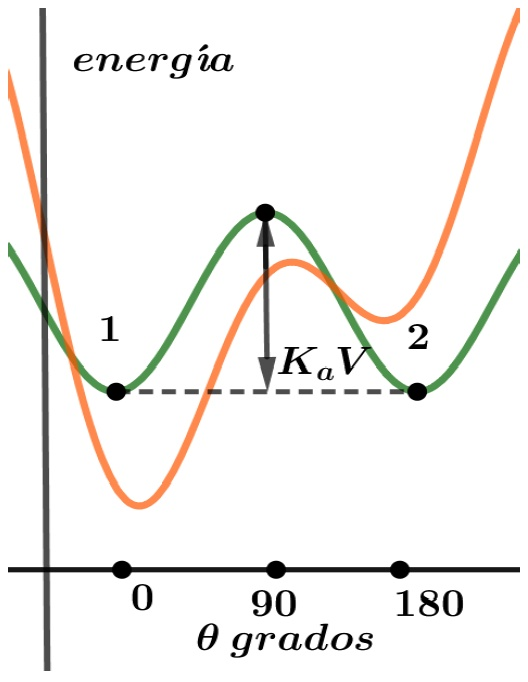
\includegraphics[width=0.4\textwidth]{./Figures/fig36}
	\caption{Proceso activado térmicamente}
	\label{fig:36}    
\end{figure}


Planteando el modelo de Bean y Livingston para el Superparamagnetismo, tenemos en la figura \ref{fig:37}, el eje de asimetría (línea verde) de una partícula con un solo dominio y el vector de magnetización En estos sistemas el comportamiento magnético observado depende del valor del tiempo típico de medición $\tau_{m}$ que emplea la técnica usada, respecto al tiempo de relajación $\tau$ propio del sistema.

\begin{figure}[H]
    \centering
    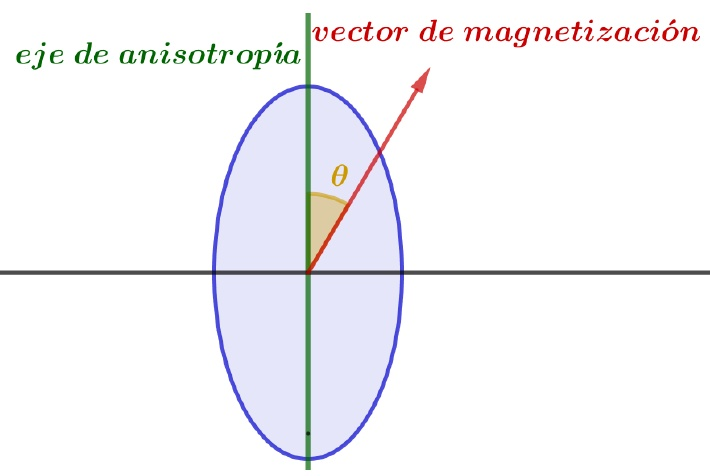
\includegraphics[width=0.6\textwidth]{./Figures/fig37}
	\caption{modelo de Bean y Livingston}
	\label{fig:37}    
\end{figure}


\begin{itemize}
	\item Si $\tau_{m}\gg \tau$ la relajación ocurre más rápido que la medición, dejando que el sistema llegue al equilibrio termodinámico. Se observa es que el conjunto de partículas se comporta de modo análogo a un sistema paramagnético.

	\item Si $\tau_{m}\ll \tau$ la relajación del sistema resulta muy lenta y se observan propiedades cuasiestáticas como
en los sistemas magnéticamente ordenados. Este régimen se denomina bloqueado.
\end{itemize}



La temperatura que divide estos dos regímenes se denomina temperatura de bloqueo $T_{B}$ y depende del tiempo característico de medición $\tau_{m}$. La temperatura de bloqueo se define como aquella en la que $\tau_{m}=\tau$ y
está asociada a la barrera de energía,. Si $\tau_{m}=\tau$ entonces:


\begin{equation}
	\tau(t)=\tau_{0} e^{\mfrac{E_{B}}{kT}} \quad \text{por lo tanto} \quad T_{B}=\mfrac{E_{B}}{k\, ln \big(\mfrac{\tau}{\tau_{m}} \big)} 
\end{equation}


\subsection{Sistemas magnéticos amorfos}


$\centerdot$ Son varias las direcciones en las que avanzaron las investigaciones y/o desarrollos en magnetismo. En esta presentación solo destacaremos algunas. Se destaca de manera especial el descubrimiento de la magnetorresistencia gigante. El caso de los cables magnéticos no es de menor importancia, dio origen a innumerables aplicaciones, ampliando aun más sus posibilidades al introducir los materiales amorfos. En la actualidad se conjugan la nanotecnología con los hilos magnéticos y las cintas amorfas. Donde surgió interés debido al descubrimiento de los fenómenos de magnetorresistencia gigante en multicapas, magnetorresistencia colosal en manganitas y la magnetoimpedancia gigante en aleaciones magnéticamente blandas en forma de hilos, cintas, películas y multicapas, en el estado amorfo, monocristalino y cristalino. Existen diferentes aplicaciones tecnológicas, principalmente en el área de la sensorística y de grabación magnética. Solo mencionamos algunos casos no diciendo nada sobre aplicaciones, de gran relevancia, en biología y medicina.

$\centerdot$  En general, como ya hemos manifestado, hay tres grupos de sistemas magnéticos; \textbf{Cintas Amorfas, Hilos Amorfos} y \textbf{Microhilos Recubiertos}. De los cuales comentaremos los dos últimos. Es conveniente recordar algunas definiciones que ya fueron comentadas: Los materiales magnetostrictivos son aquellos que se deforman bajo un campo magnético aplicado. La razón de este fenómeno es el acoplamiento entre la órbita de los electrones y su estado de espín, que provoca una elongación de la órbita en la dirección del spin. Macroscópicamente, todas las orbitas están elongadas pero en distintas direcciones del espacio. Cuando actúa un campo magnético todos los orbitales se orientan en la misma dirección y cambia de dimensión el cuerpo. Estos materiales deben sus propiedades fundamentalmente por la anisotropía magnetoelástica, que está determinada por las tensiones (mecánicas, temperatura, corrientes eléctricas) inducidas por la fabricación y la magnetostricción ($\lambda_{s}$) propia del material.

%\subsubsection{Algunos comentarios}
\subsection{Materiales magnetostrictivos}

La capacidad de deformación de los materiales magnetostrictivos, sin necesidad de contactos eléctricos los hace especialmente atractivos para fabricar microsensores y actuadores. Si bien en mayor o menor medida muchos materiales son magnetostrictivos, elementos puros como el hierro, cobalto y níquel son especialmente usados, presentan valores de $\lambda_{s}$ bajos del orden de $10ppm$, Alrededor de 1960 algunas tierras raras como el $Tb$ o $Dy$ demostraron tener extraordinarias propiedades magnetostrictivas ($\mfrac{3}{2}\lambda_{s} \sim 10000 ppm$) pero sólo a bajas temperaturas por su temperatura de Curie. En los últimos años se destaca la creación del \textbf{Terfenol-D} que oscila entre $1000$ y $2000ppm$, desarrollado para generar ondas elásticas en el agua, Sonar. En 1999 se descubre una nueva aleación capaz de soportar grandes tensiones ($\sim 500 MPa$). La aleación recibió el nombre de \textbf{Galfenol}. Aunque su magnetostricción resulta menor que las de las aleaciones anteriores, algunas de sus propiedades como: gran permeabilidad, baja histéresis, ductilidad, resistencia a impactos, y la posibilidad de ser soldados, hicieron que este material expandiera ampliamente su utilización, formando parte de sensores y actuadores. El impulso magnético debe actuar sobre el material llevándolo a saturación o próximo a ella, luego este tipo de aplicación requiere materiales con elevados valores de $\lambda_{s}$. Por otro lado, para aplicaciones en tecnologías MEMS, por ejemplo para medir campos magnéticos bajos no solo se requiere valores altos de $\lambda_{s}$ si no , también contar con alta valores de 


\begin{equation}
	\mfrac{d\lambda}{dH}
\end{equation}

además de sensibilidad y una histéresis muy pequeña y reversible. Por tanto hablamos de lo que llamamos: materiales magnéticamente blandos.


\subsection{Hilos magnéticos Amorfos}

La presencia de tensiones (mecánicas) residuales generadas en el proceso de fabricación crean, por intermedio de la magnetostricción, anisotropías magnéticas que orientan la magnetización. Las aleaciones más comunes se observa a continuación. En general los metales amorfos en forma de hilos presentan excelentes propiedades elásticas e importante resistencia mecánica. Son generalmente materiales magnéticamente blandos. En estas aleaciones se originan la anisotropía magnética por medio del acoplamiento magneto elástico, que es proporcional a la constante de magnetostricción de saturación $\lambda_{s}$ cuando actúa una tensión $\sigma$ (mecánica). Con $\lambda_{s} > 0$ (aleaciones ricas en $Fe$) la magnetización espontanea tiende a girar hacia la tensión, pudiéndose describir por la expresión de la anisotropía :

\begin{equation}
K_{\sigma} = \mfrac{3}{2}\lambda_{s}\sigma\big(Sin(\beta)\big)^{2}
\end{equation}

La representación de este fenómeno se puede ver en la figura \ref{fig:38}

\begin{figure}[H]
    \centering
    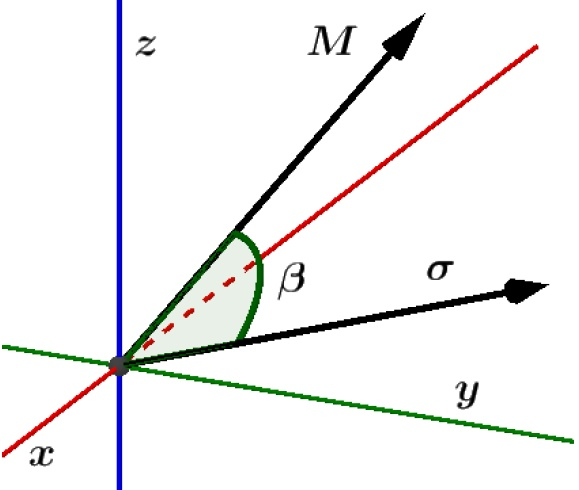
\includegraphics[width=0.5\textwidth]{./Figures/fig38}
	\caption{Hilos magnéticos Amorfos}
	\label{fig:38}    
\end{figure}

Las propiedades magnéticas de un material magnetostrictivo dependen de las tensiones mecánicas a las que está sometido

\begin{figure}[H]
    \centering
    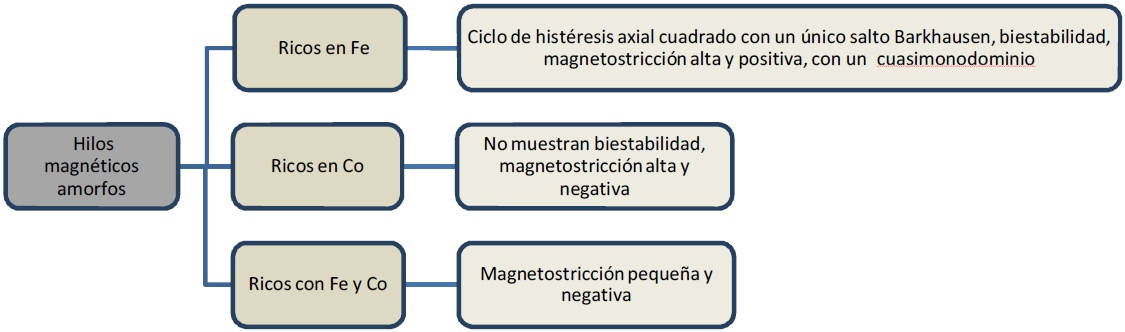
\includegraphics[width=1.1\textwidth]{./Figures/fig39}  
\end{figure}


\subsubsection{Aleaciones ricas en Fe}

\begin{figure}[H]
  \begin{minipage}[b]{0.47\textwidth}
  Como fue comentado las aleaciones ricas en con presentan un ciclo de histéresis axial cuadrado, como se observa en la figura \ref{fig:310}. El eje axial es el de fácil imanación. La inversión de la imanación o “switching” ocurre a través de un único salto Bakhausen cuando se alcanza el valor de inversión. En este caso la estructura de dominios es compuesta, por un único dominio en el núcleo con imantación axial y una corteza con varios dominios radial, Como se observa en el esquema de la figura \ref{fig:311}
  \vspace{1cm}
  \end{minipage}
  \hfill
  \begin{minipage}[b]{0.47\textwidth}
     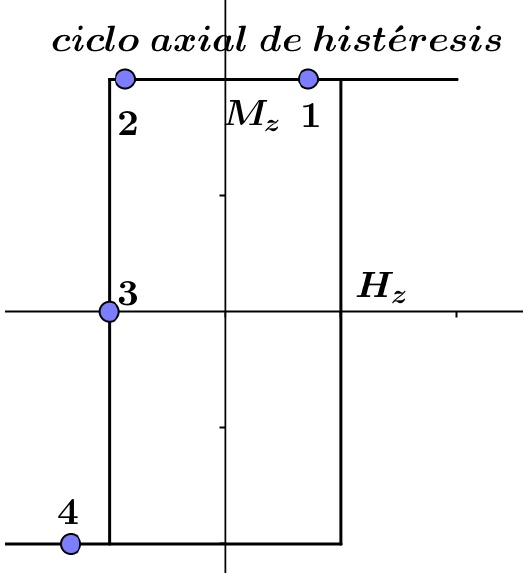
\includegraphics[width=0.9\textwidth]{./Figures/fig310}
     \caption{Ciclo de histéresis}
	\label{fig:310}
  \end{minipage}
\end{figure}

\begin{figure}[H]
    \centering
    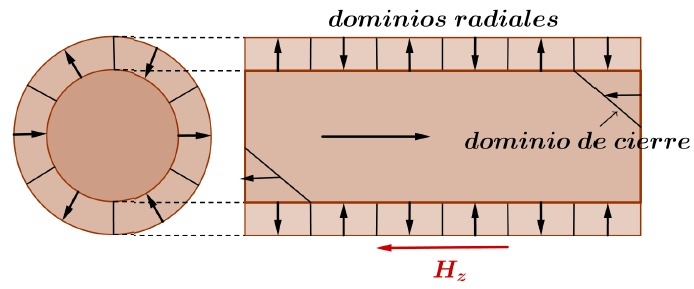
\includegraphics[width=0.6\textwidth]{./Figures/fig311}
	\caption{Distribución radial de dominios}
	\label{fig:311}    
\end{figure}




\begin{figure}[H]
  \begin{minipage}[b]{0.47\textwidth}
  La inversión de magnetización se realiza por medio del desenganche y propagación de uno de los dominios de cierre. Se observa en la figura \ref{fig:312} la variación de los dominios del núcleo cuando se aplica un campo magnético axial y opuesto a la magnetización inicial. En la etapa 2 se observa cómo se desengancha uno de los dominios de cierre.
\vspace{3cm}
  \end{minipage}
  \hfill
  \begin{minipage}[b]{0.47\textwidth}
     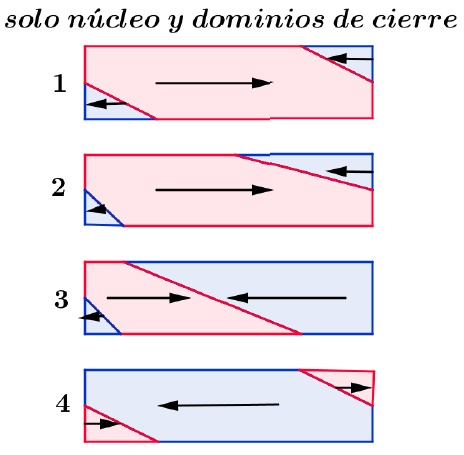
\includegraphics[width=1.10\textwidth]{./Figures/fig312}
     \caption{Inversión de magnetización}
	\label{fig:31}
  \end{minipage}
\end{figure}

En estas aleaciones ricas en $Fe$, el fenómeno de desenganche, puede observarse en la secuencia de imágenes tomadas por medio del efecto Kerr de la inversión de la magnetización. Trabajo realizado por T. Reininger, H.Kronmüller, C. Gómez-Polo, M. Vázquez, en un hilo metálico $FeSiB$ de $125\mu m$ de diámetro. El campo magnético aumenta de izquierda a derecha. En la imagen se aprecia el crecimiento de la pared del dominio del núcleo y la zona de la corteza. El proceso de inversión (\textit{switching}), de estos hilos, depende fuertemente de la longitud del hilo, lo que estaría indicando una influencia del factor desimanador asociado a la variación de la longitud del hilo.


\begin{figure}[H]
    \centering
    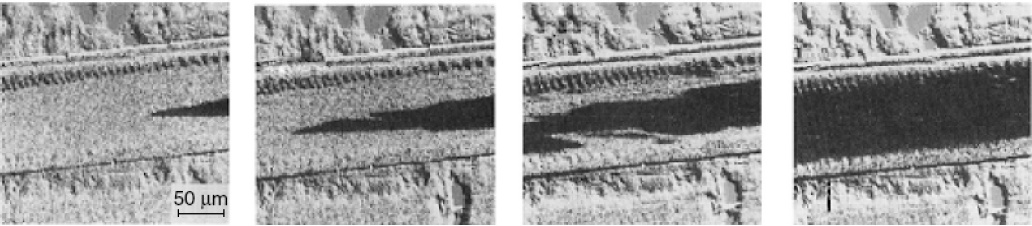
\includegraphics[width=1.0\textwidth]{./Figures/fig313}
	\caption{''Desenganche", efecto Kerr}
	\label{fig:313}
\end{figure}


Un fenómeno similar se da en los hilos ferromagnéticos amorfos recubiertos con vidrio (común).

Recordemos que la única fuente de anisotropía proviene del proceso de fabricación del metal amorfo por
causa del ultrarrápido enfriamiento del mismo, debido al gradiente de temperatura generado en el proceso. Las tensiones generadas también dependerán de las constantes elásticas del metal.

\subsection{Otros ciclos de histéresis}

Algo más sobre la susceptibilidad magnética Recordando que la magnetización o imanación $\overrightarrow{M}$ se relaciona con el campo $\overrightarrow{H}$ por medio de la expresión ${\overrightarrow{M}= \chi \overrightarrow{H}}$ donde $\chi$ es la susceptibilidad magnética. La $\chi$
depende del material, (estructura electrónica, densidad, temperatura), si el material es isótropo no depende del campo aplicado (lineal, paramagnéticos y diamagnéticos) y es un escalar; en pocas palabras significa que son colineales $\overrightarrow{M}$ y $\overrightarrow{H}$. Por el contrario si el medio es anisótropo las dos magnitudes son tensores, que en nuestro caso se representan como matrices de 3x3.

La su susceptibilidad magnética puede ser pensada como una medida de la facilidad que tiene el material a ser magnetizado por un campo magnético.

\begin{itemize}
	\item Medio isótropo ${\overrightarrow{M}= \chi \overrightarrow{H}}$
	\begin{equation}
		\overrightarrow{B}=\mu_{0}(\overrightarrow{H}+\overrightarrow{M})= \mu_{0}(\overrightarrow{H}+\chi\overrightarrow{H})= \mu_{0}(1+\chi)\overrightarrow{H}
	\end{equation}
	\item Medio anisótropo ${M_{i}= \chi_{ij} H_{j}}$
	\begin{equation*}
	\begin{split}
		B_{i} & =\mu_{0}(H_{i}+M_{i})=\mu_{0}(H_{i}+\chi_{ij}H_{j})\\
		      & =\mu_{0}(H_{j}\delta_{ij}+\chi_{i}H_{j})=\mu_{0}(\delta_{ij}+\chi_{ij})H_{j} \\
	\end{split}
	\end{equation*}
	
	\begin{equation}
\begin{pmatrix}
B_{1}\\
B_{2}\\
B_{3}
\end{pmatrix}		
=
\begin{pmatrix}
1+ \chi_{11} & \chi_{21} & \chi_{31} \\
\chi_{12} & 1+\chi_{} & \chi_{32} \\
\chi_{13} & \chi_{23} & 1+\chi_{33}
\end{pmatrix}		
\begin{pmatrix}
H_{1}\\
H_{2}\\
H_{3}
\end{pmatrix}		
	\end{equation}	
	 
\end{itemize}

El tensor $\chi_{ij}$ es simétrico lo que implica que $\chi_{ij}=\chi_{ji}$ y de coeficientes reales por tanto el tensor puede ser diagonalizado y ser escrito como


\begin{equation}
\begin{pmatrix}
\chi_{1} & 0 & 0 \\
0 & \chi_{2} & 0 \\
0 & 0 & \chi_{3}
\end{pmatrix}		
\end{equation}

Donde $\chi_{n}$ son las componentes principales del tensor. Como todo tensor de segundo orden puede ser representado por una cuádrica.

En general, la magnetización $\overrightarrow{M_{s}}$ formará unos ángulos $\alpha$, $\beta$ , $\theta$ con los ejes de coordenadas, si trabajamos en cilíndricas los vectores unitarios son $u_{r}$, $u_{\varphi}$, $u_{z}$, respectivamente. Las componentes de la magnetización respecto a esos ejes son: $M_{r}=M_{s}Cos(\alpha)$, $M_{\varphi}=M_{s}Cos(\beta)$ y $M_{z}=M_{s}Cos(\theta)$.

Generalmente hay dos tipos de campos magnéticos externos que pueden $H_{z}$ y $H_{\varphi}$ son los campos axial y circular. Veamos este caso con el tensor aplicado a una muestra:


$\centerdot$ Axial $\overrightarrow{H_{z}}=Hu_{z}$, por medio de un solenoide. Si la muestra es un hilo el campo es constante a lo largo del hilo.
	
$\centerdot$ Circunferencial $\overrightarrow{H_{\varphi}}=Hu_{\varphi}$. Producido por una corriente eléctrica que circula a lo largo de la muestra, por ejemplo de un hilo. En este caso el campo no es constante en la sección del hilo, aumenta linealmente con $r$, de acuerdo a la expresión:

\begin{equation*}
H=\mfrac{I\, r}{2\pi R^{2}}
\end{equation*}

Siendo $R$ el radio del hilo e $I$ la corriente. De acuerdo a como coloquemos el campo magnético y que $M$ midamos tendremos distintos ciclos de histéresis, por ejemplo:
\begin{itemize}
\item{1} Axial, $M_{x}$ en función de $H_{z}$

\item{2} Circunferencial, $M_{\varphi}$ en función de $H_{\varphi}$.

\item{3} Termino no diagonal del tensor del tensor de susceptibilidad $M_{\varphi}$ en función de $H_{z}$ o $M_{z}$ en función de $H_{\varphi}$.

\end{itemize}

En los hilos de simetría cilíndrica y amorfos la magnetización tiene componentes radial, circular y axial. Si solo tomamos en cuenta las componentes radial y circular $M_{z}$ y $M_{\varphi}$. Si:

	\begin{equation}
\begin{pmatrix}
M_{z}\\
M_{\varphi}
\end{pmatrix}		
=
\begin{pmatrix}
\chi_{zz} & \chi_{z\varphi1} \\
\chi_{\varphi z} & \chi_{\varphi\varphi} 
\end{pmatrix}		
\begin{pmatrix}
H_{z}\\
H_{\varphi}
\end{pmatrix}		
	\end{equation}	

\begin{figure}[H]
    \centering
    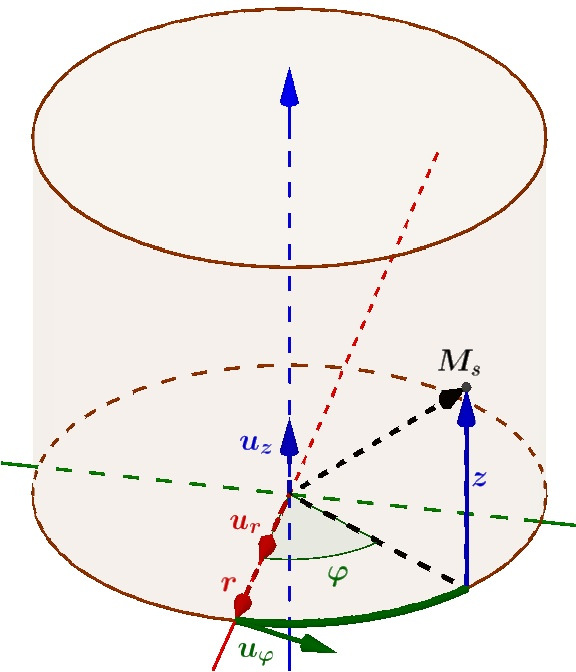
\includegraphics[width=0.5\textwidth]{./Figures/fig314}
	\caption{Coordenadas cilíndricas}
	\label{fig:314}
\end{figure}

\textbf{Luego el campo axial puede influir sobre las componentes axial y circular de la magnetización}, esta influencia está dada por los términos no diagonales de la matriz. A este respecto, hay dos efectos, que comentamos anteriormente que se encuentran relacionados con los términos no diagonales de la matriz estos son; el \textbf{efecto Matteucci} y el \textbf{efecto Wiedemann} inverso. Para lograr estos efectos debe existir una anisotropía cuya dirección forme un ángulo entre la dirección del campo y la de la dirección de magnetización. Una forma de lograr esto es sometiendo al cable a torsión. Esta deformación logra direcciones de fácil magnetización helicoidales, o sea a $45^{o}$ con la dirección axial y circular.


\subsubsection{Aleaciones ricas en Co}

\begin{figure}[H]
  \begin{minipage}[b]{0.47\textwidth}
Estas aleaciones tienen magnetostricción negativa y alta, del orden de $-10^{-6}$, su ciclo de histéresis axial se puede observan en la figura \ref{fig:315}. La estructura de dominios en estos microhilos rico en cobalto es circular, como observamos en la figura \ref{fig:316}. Tanto la estructura de dominios como el ciclo de histéresis depende del proceso de fabricación. Al incrementar el campo aplicado rota la magnetización de manera cuasireversible desde la dirección circunferencial hasta la axial, generando el ciclo de histéresis particular que se observa en la figura.
  \vspace{0.2cm}
  \end{minipage}
  \hfill
  \begin{minipage}[b]{0.47\textwidth}
     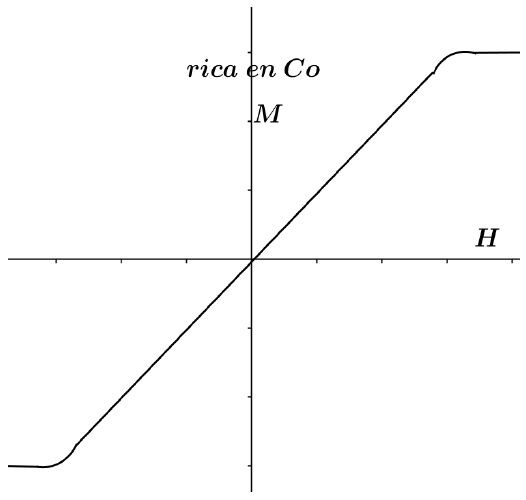
\includegraphics[width=1.0\textwidth]{./Figures/fig315}
     \caption{Histéresis axial}
	\label{fig:315}
  \end{minipage}
\end{figure}

\begin{figure}[H]
    \centering
    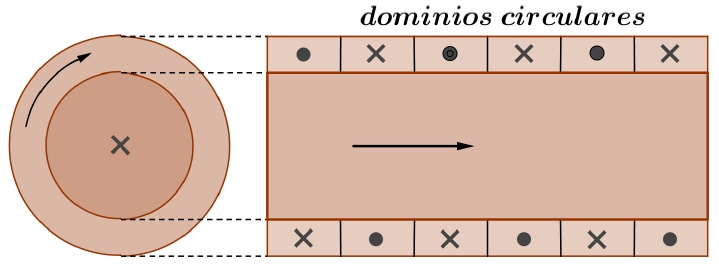
\includegraphics[width=0.6\textwidth]{./Figures/fig316}
	\caption{Estructura del microhilo}
	\label{fig:316}
\end{figure}


\section{Magnetoresistencia (MR)}

Es la propiedad que posee algunos materiales por la cual cambian su resistencia eléctrica cuando actúa sobre ellos un campo magnético externo.


\subsection{MR Anisótropa}

En 1856-1857 que Thomson (Lord Kelvin) descubrió un fenómeno, denominado Magnetoresistencia Anisotrópica, al medir la resistencia eléctrica de $Fe$ y $Ni$ en presencia de un campo magnético. Kelvin informo un incremento en la resistencia de 0.2\%, cuando el campo magnético era aplicado en la dirección de la corriente y un decrecimiento de 0.4\%, cuando el campo era aplicado en la dirección transversal. Posteriormente, esto fue explicado en términos de la interacción espín-órbita. Puesto que el electrón poseía un momento magnético cuyo vector buscaría alinearse o antialinearse con la dirección del campo magnético aplicado. Los orbitales de los átomos de la red son centros de dispersión para los electrones de conducción. Como también las impurezas, defectos estructurales y otros electrones.


Al aplicarse un campo magnético externo se reorientan los spines variando los procesos de dispersión y por tanto cambia la resistencia. Cuando mayor es la sección que opone el átomo de la red mayor será la dispersión y por tanto, mayor la resistencia. Recordemos, en la figura \ref{fig:317}, uno de los orbitales $3d^{6}$ para el $Fe$.

En general este efecto es observado en metales de transición $3d$ y sus aleaciones y responden, en la mayoría de los casos, a la siguiente expresión:

\begin{equation}
	\rho(\theta)=\rho_{\perp}+(\rho_{\parallel}-\rho_{\perp})Cos^{2}(\theta)
\end{equation}

Donde $\rho_{\perp}$ y $\rho_{\parallel}$ son las resistencias a $\theta=90^{o}$ y $\theta=0^{o}$ ,siendo $\theta$ el ángulo entre el campo y la corriente.


\begin{figure}[H]
    \centering
    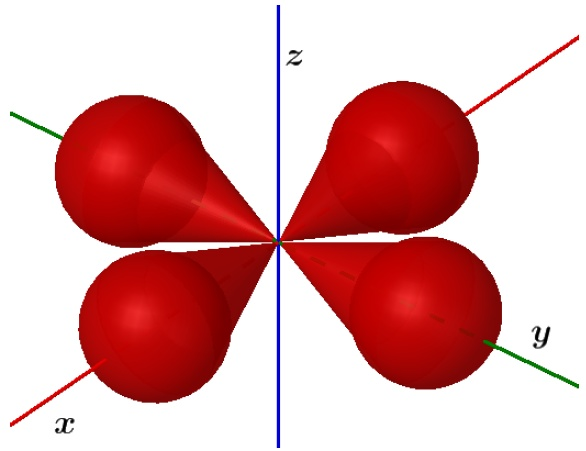
\includegraphics[width=0.5\textwidth]{./Figures/fig317}
	\caption{Orbitales $3d$}
	\label{fig:317}
\end{figure}

Las investigaciones recientes han permitido descubrir materiales que presentan magnetorresistencia gigante (\textit{Giant Magnetoresistance Effect}, o GMR), magnetorresistencia colosal (\textit{Colossal Magnetoresistance} o CMR) y magnetorresistencia de efecto túnel (\textit{Tunnel Magnetoresistance Effect} o TMR). Tanto la MR como la GMR se basan en el espín de los electrones y por eso forman parte de la espintrónica.

\begin{figure}[H]
    \centering
    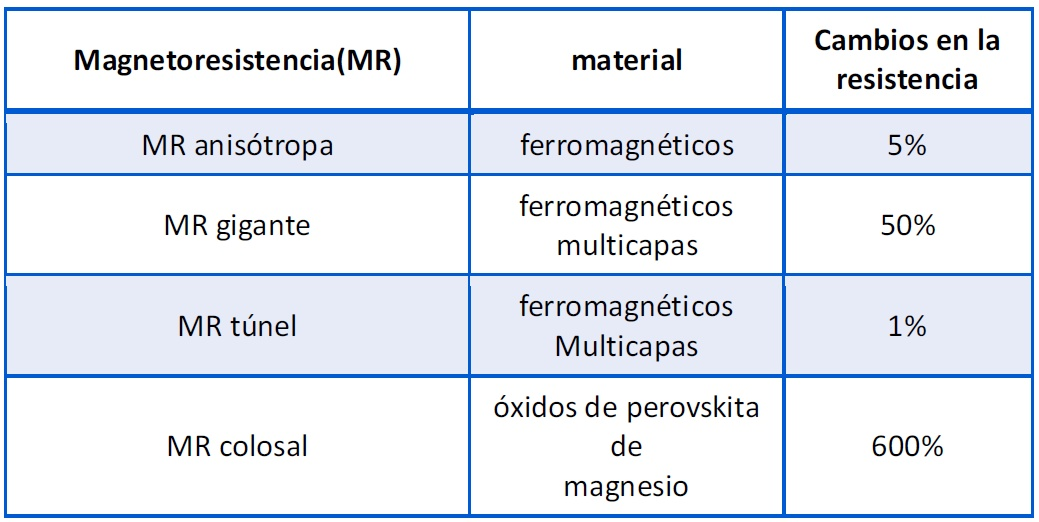
\includegraphics[width=0.9\textwidth]{./Figures/fig318}
	\label{fig:318}
\end{figure}

\subsection{Conductividad eléctrica}

Comentaremos un poco más el fenómeno de la Magnetoresistencia Anisotrópica. Queremos llegar a demostrar elementalmente que

\begin{equation}
	\mfrac{R(H)-R(0)}{R(0)}\approx Cta(H^{2})
\end{equation}

o sea, que la variación relativa de la resistencia depende del campo aplicado al cuadrado.

Supongamos que en un metal tenemos $n$ electrones por unidad de volumen. En ausencia de campo eléctrico exterior la velocidad media de los electrones es cero $\bar{\overrightarrow{v}}=\mfrac{1}{n}\sum_{i=1}^{n} \overrightarrow{v_{i}}$, el mismo número de electrones se mueve en una dirección como en la opuesta. Cuando aplicamos un campo eléctrico la velocidad media deja de ser cero y los electrones se mueven libremente hasta que colisionan con algún centro de dispersión. El tiempo que transcurre entre colisiones se llama tiempo de relajación $\tau$. Llamamos $\overrightarrow{J}$ a la densidad de corriente que es la carga eléctrica transportada por unidad de tiempo y área $\overrightarrow{J}=n\,e\,\overrightarrow{v}$. La ecuación de movimiento de los electrones es:

\begin{equation}
	m\big(\mfrac{d\overrightarrow{V}}{dt}+\mfrac{1}{\tau} \overrightarrow{v} \big)= e\, \overrightarrow{E}
\end{equation}

Si la velocidad de traslación no varía con el tiempo, la solución será:

\begin{equation}
	\overrightarrow{v} = \mfrac{e\,\tau}{m} \overrightarrow{E} = \mu \overrightarrow{E}
\end{equation}

Calculemos la densidad de corriente en función de la velocidad media $\overrightarrow{J}=n\,e\,\overrightarrow{v} = n\,e\,\mu \,\overrightarrow{E}$, que es la ley de Ohm, por tanto $\overrightarrow{J}=\sigma \overrightarrow{E}$ siendo $\sigma$ la conductividad eléctrica y $\rho=\sigma^{-1}$ la resistividad.

Recordando que $E=\mfrac{V}{L}$, donde $L$ es longitud y $V$ la diferencia de potencial , como $J=\mfrac{I}{A}$ con $I$ corriente y $A$ área, luego la resistencia eléctrica la podemos escribir, reemplazando:

\begin{equation}
	R= \mfrac{V}{I}= \mfrac{El}{JA}= \mfrac{EL}{\sigma E A}= \mfrac{L}{\sigma A}
\end{equation}

Veamos el caso para Conductividad Eléctrica y Magnetoresistencia “normal”:

Si introducimos un campo magnético externo, los electrones viajan de manera individual en trayectorias onduladas, La componente magnética de la fuerza de Lorentz ($\overrightarrow{f}=e \overrightarrow{v}\wedge\overrightarrow{H}$) provoca este comportamiento de los electrones haciendo que viajen una distancia mayor y a su vez, incrementando la cantidad de eventos de dispersión. 

Sabemos de mecánica que:

\begin{figure}[H]
  \begin{minipage}[b]{0.47\textwidth}
\begin{equation*}
\begin{split}
	\overrightarrow{f} & = -e\overrightarrow{v} \wedge \overrightarrow{H}  \therefore f= evH = ma = m\omega^{2}r \\
	 & \omega^{2}r = \mfrac{evH}{m}	 = \mfrac{e\omega r H}{m} \\
	 & \omega = \mfrac{eH}{m} \\
	\theta & = \omega\tau= \mfrac{eH}{m}\tau=\mfrac{e\tau}{m} H	 = \mu H 
\end{split}
\end{equation*}  
  \vspace{0.0cm}
  \end{minipage}
  \hfill
  \begin{minipage}[b]{0.47\textwidth}
     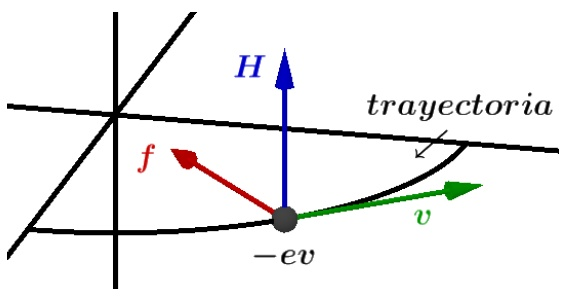
\includegraphics[width=0.9\textwidth]{./Figures/fig319}
	\label{fig:319}
	  \vspace{0.0cm}
  \end{minipage}
\end{figure}

Continuando el análisis de la figura \ref{fig:320} se deduce que:

\begin{equation*}
\begin{split}
	L_{1}= & 2rSin(\mfrac{\theta}{2} \approx 2r\big( \mfrac{\theta}{2} -\mfrac{\theta^{3}}{8} \big), \text{luego será:} \\ 	
	 & \mfrac{L_{0}-L_{1}}{L_{0}}=\mfrac{\Delta L}{L_{0}} \approx \theta^{2}	
\end{split}
\end{equation*}  

\begin{figure}[H]
    \centering
    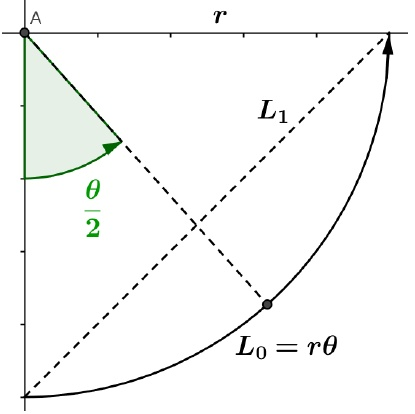
\includegraphics[width=0.4\textwidth]{./Figures/fig320}
	\caption{Momento angular}
	\label{fig:320}
\end{figure}

Por otro lado tenemos que $R=\mfrac{L}{\sigma A}$ y entonces será:

\begin{equation}
	\mfrac{R(H)-R(0)}{R(0)} = \mfrac{\Delta L}{L_{0}} \approx (\mu H)^{2}
\end{equation}

Expresión esta última que es la magnetoresistencia “normal”, de acuerdo con los datos experimentales.

\subsection{MR por magnetización espontánea}

En metales no magnéticos, la resistencia eléctrica decae suavemente a medida que disminuye la temperatura. Este comportamiento es debido a la disminución de las vibraciones térmicas de los átomos. Como consecuencia de esto, la dispersión de los electrones es menor.

Si el metal es ferromagnético, existe una reducción adicional en la resistencia, debida a la alineación de los momentos magnéticos, (en ciertas circunstancias), a medida que se reduce la temperatura, que resulta en una disminución de la dispersión de los electrones de conducción, esto se representa en la figura \ref{fig:321}

\begin{figure}[H]
    \centering
    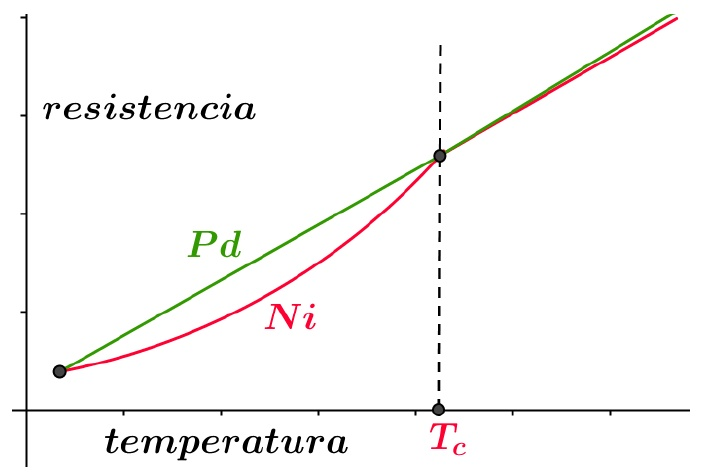
\includegraphics[width=0.5\textwidth]{./Figures/fig321}
	\caption{Resistencia - temperatura}
	\label{fig:321}
\end{figure}


\subsection{MR Gigante}

Es en 1988 la fecha en que Albert Fert y Peter Grünberg demuestran por separado, la existencia de un fenómeno llamado magnetoresistencia gigante, por lo cual les dieron el premio Nobel de física en el año 2007. La magnetoimpedancia gigante se observado en materiales ferromagnéticos blandos y consiste en una gran variación de la impedancia alterna, ${Z= R(\omega, H_{cc}) + iX(\omega, H_{cc})}$, cuando se hace pasar, por el material ferromagnético, una corriente alterna $I_{ac}$ de frecuencia $\omega$ en presencia de un campo magnético continuo $H_{cc}$. Fundamentalmente esta causada por la distribución no uniforme de la corriente alterna, efecto pelicular o “\textit{skin}” el cual fue mencionado anteriormente y se describe en términos de la  penetración $\delta$ del campo electromagnético en el conductor:


\begin{equation}
	\delta= \sqrt{\mfrac{2}{\omega\sigma\mu}}
\end{equation}

Siendo $\mu$ la permeabilidad magnética y $\sigma$ la conductividad. Vemos que la penetración al cuadrado es inversamente proporcional a $\omega$, la frecuencia, conductividad y permeabilidad magnética. Este fenómeno tiene una influencia directa sobre la impedancia, ya que, está no dependerá del área total del conductor, sino solo de la región donde circula la corriente, que es menor, dependiendo como vimos, de $\delta$. Si la frecuencia del campo no varía y $\sigma$ la conductividad permanece constante, la impedancia solo dependerá de la permeabilidad magnética. Aquí, debemos ser cuidadosos al mencionar la permeabilidad, ya que sabemos de su carácter tensorial, luego si la probeta es plana la permeabilidad debería ser la transversal, mientras que si hablamos de hilos debería ser la permeabilidad circunferencial, que controlara a la impedancia. Pero, recordemos que la permeabilidad magnética depende del campo magnético exterior.

La variación típica de la impedancia en micro-hilos es de dos tipos según que el material sea:

\begin{itemize}
	\item Rico en $Fe$ con anisotropía magnética axial. 
	\item Rico en $Co$ con anisotropía magnética transversal.
\end{itemize}

Veamos el primer caso: Rico en $Fe$, con anisotropía magnética axial (longitudinal, paralela al eje del hilo, $\lambda_{s}>0$ ).



\begin{figure}[H]
  \begin{minipage}[b]{0.47\textwidth}
En este caso la impedancia presenta un solo pico, como es observado en la figura \ref{fig:322}, con un máximo de la impedancia cuando $H_{cc}$ es cero. El material posee una anisotropía magnética en la dirección de circulación de la corriente y coincide con la dirección del campo magnético. En este caso la muestra ya se encuentra saturada axialmente con $H_{cc}=0$ luego un aumento $H_{cc}$ de fijara más $M$ desplazando las paredes de los dominios hasta que solo prevalezca un solo dominio y la permeabilidad circunferencial solo puede disminuir.
  \vspace{1.5cm}
  \end{minipage}
  \hfill
  \begin{minipage}[b]{0.47\textwidth}
     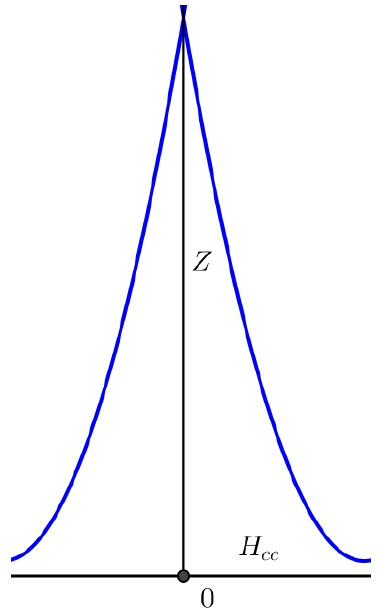
\includegraphics[width=0.8\textwidth]{./Figures/fig322}
	\label{fig:322}
	  \vspace{0.0cm}
  \end{minipage}
\end{figure}

Tendremos dos estados:

El estado inicial con $H_{cc}=0$ con dos dominios
\begin{figure}[H]
    \centering
    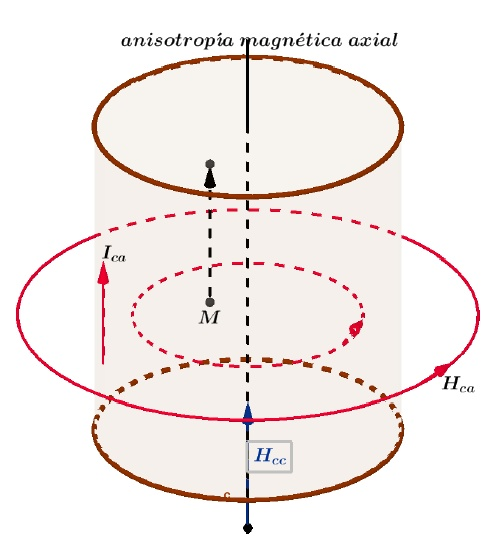
\includegraphics[width=0.5\textwidth]{./Figures/fig323}
	\caption{Un solo dominio}
	\label{fig:323}
\end{figure}

y el estado final con un solo dominio

\begin{figure}[H]
    \centering
    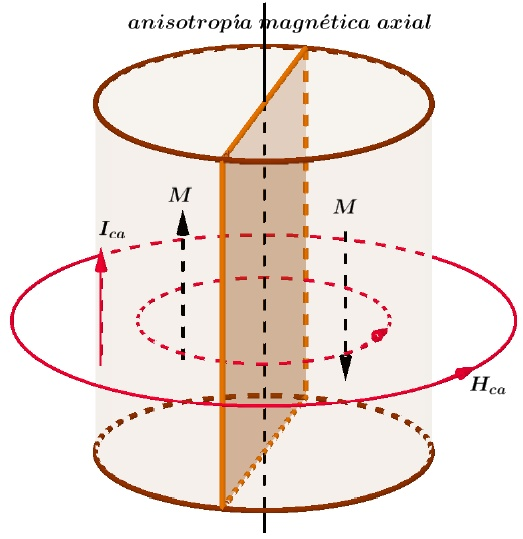
\includegraphics[width=0.5\textwidth]{./Figures/fig324}
	\caption{Dos dominios}
	\label{fig:324}
\end{figure}

El segundo caso: Rico en $Co$,con anisotropía magnética transversal $\lambda_{s}<0$ será:

\begin{figure}[H]
  \begin{minipage}[b]{0.47\textwidth}
Sin campo continuo $H_{cc}=0$ las variaciones de $H_{ca}$ tienen muy poca influencia sobre la magnetización $M$ transversal. Si se aplica un campo $H_{cc}$ pequeño la posición de equilibrio de se modifica y la magnetización oscilara de acuerdo a la corriente alterna incrementando $\mu_{t}$ En la medida que aumenta $H_{cc}$, $M$ se
aproxima mas a la dirección axial y aumenta $\mu_{t}$ Cuando es igual al campo de anisotropía $\pm H_{k}$ se produce el máximo de $\mu_{t}$ y cualquier aumento posterior de $H_{cc}$ produce una disminución de $Z$.
  \vspace{1.0cm}
  \end{minipage}
  \hfill
  \begin{minipage}[b]{0.47\textwidth}
     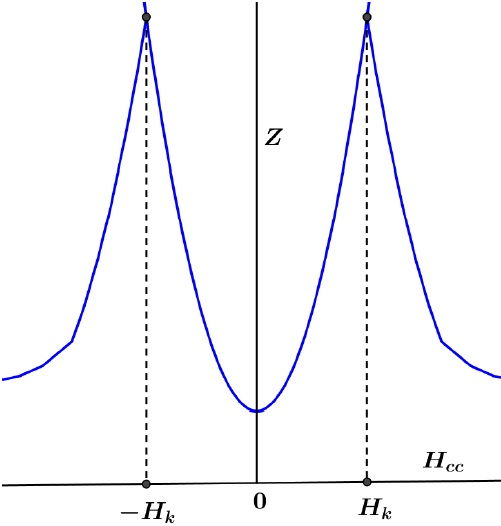
\includegraphics[width=1.0\textwidth]{./Figures/fig325}
	\label{fig:325}
	  \vspace{0.0cm}
  \end{minipage}
\end{figure}

\subsection{Anisotropía Magnética Transversal}

Se observan en los esquemas dos dominios magnéticos con anisotropía trasversal.

\begin{figure}[H]
  \begin{minipage}[b]{0.47\textwidth}
 Vemos que al aumentar el campo $H_{cc}$ el campo $H_{ac}$ hace oscilar el momento magnético $M$ alrededor de $H_{cc}$
  \vspace{1cm}
  \end{minipage}
  \hfill
  \begin{minipage}[b]{0.47\textwidth}
     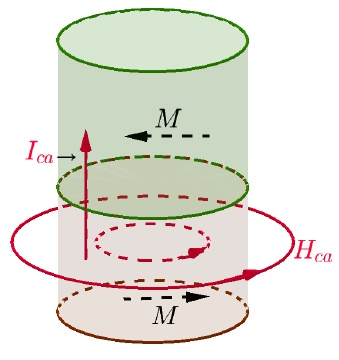
\includegraphics[width=0.8\textwidth]{./Figures/fig326}
	\label{fig:326}
  \end{minipage}
\end{figure}

\begin{figure}[H]
  \begin{minipage}[b]{0.47\textwidth}
     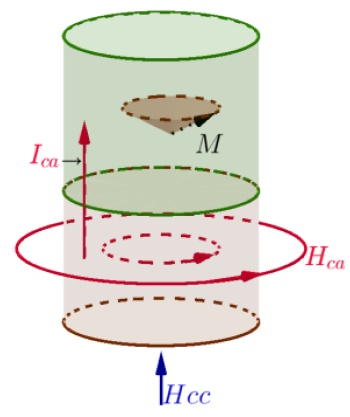
\includegraphics[width=0.8\textwidth]{./Figures/fig327}
	\label{fig:327}
  \end{minipage}
  \hfill
  \begin{minipage}[b]{0.47\textwidth}
Cuando $H_{cc}$ llega a valer $H_{k}$ el momento magnético es colineal con el campo exterior.
  \vspace{2cm}
  \end{minipage}
\end{figure}

\begin{figure}[H]
  \begin{minipage}[b]{0.47\textwidth}
Llamamos a $H_{k}$ campo de anisotropía y es el campo efectivo con magnitud tal que
ejerce la misma rotación sobre $M$ que la anisotropía del material.
  \vspace{2cm}
  \end{minipage}
  \hfill
  \begin{minipage}[b]{0.47\textwidth}
     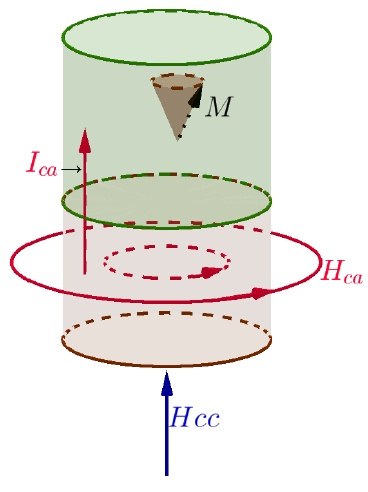
\includegraphics[width=0.8\textwidth]{./Figures/fig328}
	\label{fig:328}
  \end{minipage}
\end{figure}

\begin{figure}[H]
  \begin{minipage}[b]{0.47\textwidth}
     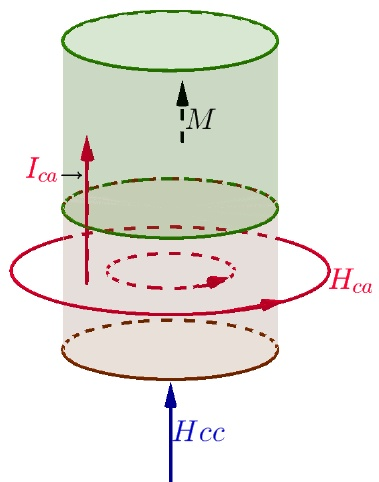
\includegraphics[width=0.8\textwidth]{./Figures/fig329}
	\label{fig:329}
  \end{minipage}
  \hfill
  \begin{minipage}[b]{0.47\textwidth}
A partir de $H_{k}$ la impedancia comienza a disminuir.
  \vspace{3cm}
  \end{minipage}
\end{figure}

A los efectos de una mejor comprensión de los temas siguientes, conviene hacer aquí un pequeño paréntesis y desarrollar los temas de resonancia ferromagnética y corriente de espín.

\section{Resonancia Ferromagnética}

La resonancia ferromagnética, observada por primera vez por Griffiths en 1946, ocurre cuando un material ferromagnético es puesto en presencia de un campo magnético. Recordemos que los átomos ferromagnéticos poseen un momento magnético neto dado por sus electrones no apareados. Si sobre un átomo ferromagnético actúa un campo magnético exterior $H_{cc}$ continuo, los momentos magnéticos de los electrones comienzan a precesar alrededor del campo (ver figura \ref{fig:330}) con una frecuencia dada por la expresión de Larmor, como ya fue comentado. La posición de equilibrio del momento magnético de un átomo $\overrightarrow{\mu}$ en el campo magnético externo es la dirección paralela al campo, como lo muestra la expresión:

\begin{equation}
	\overrightarrow{\tau}= \overrightarrow{\mu}\wedge \overrightarrow{M}
\end{equation}

\begin{figure}[H]
    \centering
    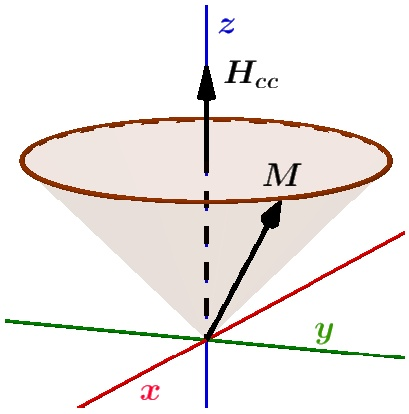
\includegraphics[width=0.4\textwidth]{./Figures/fig330}
	\caption{Campo perpendicular}
	\label{fig:330}
\end{figure}

En presencia de un campo perpendicular o por agitación térmica, el momento magnético $\overrightarrow{\mu}$ comenzará a precesar en torno a $H_{cc}$ (ver figura \ref{fig:331}) saliendo del equilibrio. Luego, el torque $\overrightarrow{\tau}$, genera una variación del momento angular (ojo, momento angular del electrón). $\overrightarrow{\tau}=\mfrac{d\overrightarrow{L}}{dt}$ o bien como $\overrightarrow{L}=h\overrightarrow{S}$, reemplazando:

\begin{equation}
	\mfrac{d\overrightarrow{S}}{dt}=\overrightarrow{\mu} \wedge \overrightarrow{H_{cc}}= \mfrac{-g \mu_{B}}{h} \overrightarrow{S} \wedge \overrightarrow{H_{cc}}
\end{equation}

Y haciendo $\mfrac{-g \mu_{B}}{h} = \gamma$  queda:

\begin{equation}
	\mfrac{d\overrightarrow{S}}{dt}= \gamma \overrightarrow{S} \wedge \overrightarrow{H_{cc}}
\end{equation}

Expresión que indica cómo el spin precesa en torno al campo magnético.

\begin{figure}[H]
    \centering
    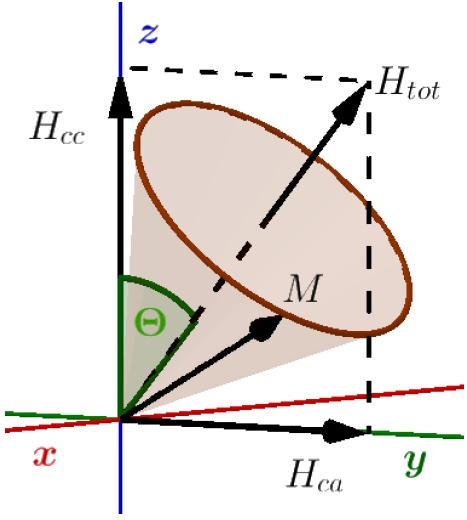
\includegraphics[width=0.4\textwidth]{./Figures/fig331}
	\caption{Precesión alrededor de $H_tot$}
	\label{fig:331}
\end{figure}

Lo expuesto es solo para un electrón pero un material ferromagnético posee gran cantidad de átomos con las características expuesta. Dicho de otro modo, todos los momentos magnéticos alineados en torno al campo aplicado. Es posible calcular la magnetización macroscópica $\overrightarrow{M}$, será

\begin{equation}
	\overrightarrow{M}=\mfrac{1}{V} \sum_{\forall i} \overrightarrow{\mu_{i}} 
\end{equation}

Donde $V$ es el volumen de la muestra. Luego la ecuación de movimiento de la magnetización será:

\begin{equation}
	\mfrac{d\overrightarrow{M}}{dt}=-\gamma \overrightarrow{M}\wedge \overrightarrow{H_{cc}} 
\end{equation}

\begin{figure}[H]
    \centering
    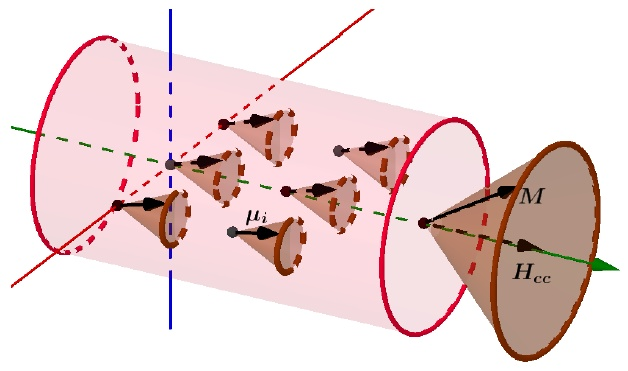
\includegraphics[width=0.4\textwidth]{./Figures/fig332}
	\caption{Precesión de la $M$ total alrededor de $H_tot$}
	\label{fig:332}
\end{figure}

Si ahora se introduce un nuevo campo magnético, pero alterno $H_{ca}$ y perpendicular a $H_{cc}$ (ver figura \ref{fig:333}, la magnetización precesará alrededor de la suma de ambos campos $H_{tot}$, formando un ángulo $\theta$ con $H_{cc}$. Si aumentamos la frecuencia de $H_{ca}$, el ángulo $\theta$ se incrementa. Cuando nos aproximamos a $\omega_{0}$, frecuencia de Lamor, $H_{tot}$ es perpendicular a $H_{cc}$.
Este fenómeno se llama \textbf{Resonancia Ferromagnetica}.

Calculemos el valor de $\omega_{0}=\gamma H_{cc}$, como $\gamma=\mfrac{g\mu_{b}}{\hbar}$ para $g=2$ es $2\pi\,2,8 \frac{GHz}{KOe}$, luego para un campo de algunos $KOe$, $1Oe= \frac{1000}{4\pi}\left[\frac{A}{m} \right]$ la frecuencia estaría en la zona de las microondas.

\begin{figure}[H]
    \centering
    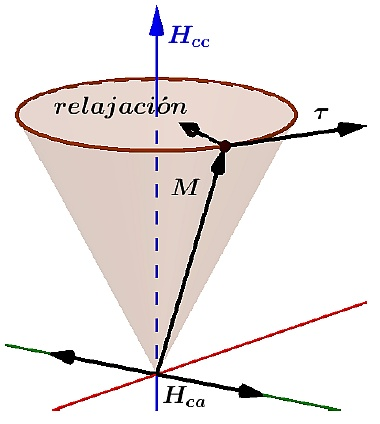
\includegraphics[width=0.4\textwidth]{./Figures/fig333}
	\caption{Relajación de la $M$ total}
	\label{fig:333}
\end{figure}

El problema de determinar la frecuencia de resonancia $\omega_{0}$ es un poco mas complicado de lo aquí expuesto, pues, existe según la forma de la muestra un campo de desmagnetización que se opone al campo aplicado, también la anisotropía lo modifican. Luego la frecuencia depende de varios factores, en general los mecanismos mencionados son de perdidas o relajación y son descritos fenomenológicamente. Por tanto la expresión de la ecuación de movimiento de la magnetización se debe modificar agregando un segundo término, sin entrar en detalles.


\begin{equation*}
	\mfrac{d\overrightarrow{M}}{dt}=-\gamma \overrightarrow{M}\wedge \overrightarrow{H_{cc}} + \text{términos de relajación}
\end{equation*}

\begin{figure}[H]
  \begin{minipage}[b]{0.47\textwidth}
Esta expresión es conocida con el nombre de Landau-Lifshtz-Gilbert. La potencia de la señal de microonda absorbida por la muestra. $P_{abs}$ se mide en función del campo de continua $\overrightarrow{H_{cc}}$ presentando un máximo en resonancia, como se observa en la figura.
  \vspace{1.5cm}
  \end{minipage}
  \hfill
  \begin{minipage}[b]{0.47\textwidth}
     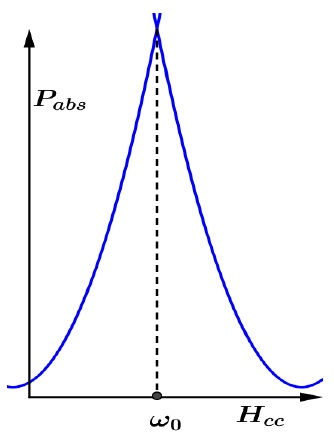
\includegraphics[width=0.8\textwidth]{./Figures/fig334}
	\label{fig:334}
	  \vspace{0.0cm}
  \end{minipage}
\end{figure}

\subsection{Corriente de espín}

Los electrones se caracterizan por sus propiedades intrínsecas: \textbf{masa}, \textbf{carga eléctrica} y \textbf{espín}, (nunca dejan de tenerlas). La carga eléctrica es la que se ha dado origen a la electricidad y electrónica convencional.
Hasta hace pocos años no se tenia en cuenta el espín en una corriente eléctrica. Tampoco era necesario preguntarse por el espín cuando los conductores eran el cobre o la plata. Si el conductor es un material ferromagnético hay una interacción entre el espín y el campo magnético del conductor dando origen a la corriente de espín. Esta nueva área de la Física es llamada espintrónica o magnetolectrónica.

La corriente de espín tiene encuentra la orientación del espín pero también puede estar asociada con la corriente de carga, se puede tener un flujo de corriente de carga con espines polarizados, como se verá en posteriores desarrollos. La corriente de espín se puede pensar como la diferencia entre el flujo de los espines hacia arriba y los espines hacia abajo. Como se observa en el esquema.

\begin{figure}[H]
    \centering
    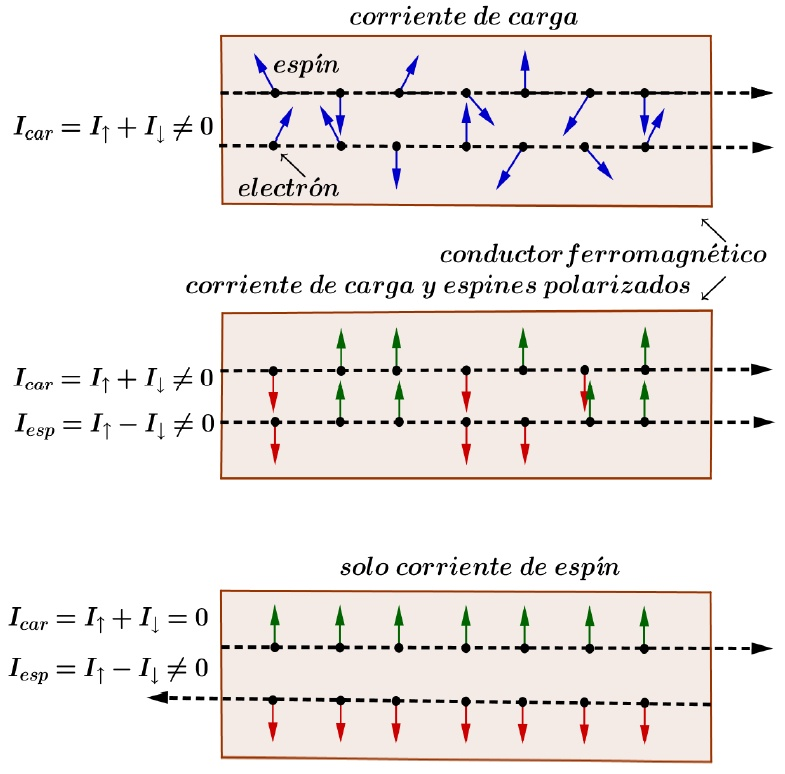
\includegraphics[width=0.8\textwidth]{./Figures/fig335}
	\caption{Corriente de espín}
	\label{fig:335}
\end{figure}

\subsection{Válvula de espín(ferromagnéticos multicapas)}
Antes de pasar a la magnetorresistencia de efecto túnel veremos la denominada \textbf{válvula de espín}.




\begin{figure}[H]
  \begin{minipage}[b]{0.47\textwidth}
Estas están formadas por dos capas ferromagnéticas separadas por un material metálico que no es ferromagnético de un espesor de aproximadamente $1nm$, por ejemplo $FeCrFe$ La capa ferromagnética de la izquierda la llamamos $Fe_{1}$ y a la de la derecha $Fe_{2}$ Una de las capas presenta una magnetización fija mientras que la otra la podemos variar con el campo externo $H_{ext}$ Obsérvese que dibujamos la corriente que incide sobre $Fe_{1}$ como si fueran dos, cada una con un tipo de espín. Estas
corrientes cuando atraviesan el material se separan.
  \vspace{0cm}
  \end{minipage}
  \hfill
  \begin{minipage}[b]{0.47\textwidth}
     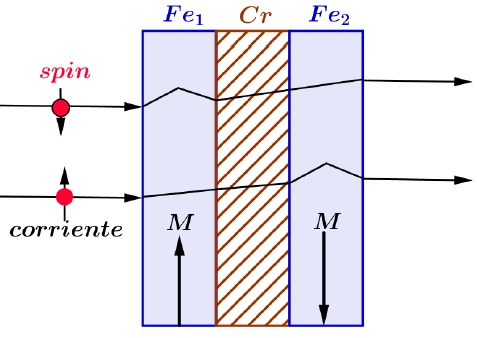
\includegraphics[width=1.0\textwidth]{./Figures/fig336}
	\label{fig:336}
	  \vspace{1.5cm}
  \end{minipage}
\end{figure}


\begin{figure}[H]
  \begin{minipage}[b]{0.47\textwidth}
Cada electrón, dependiendo de la orientación de su espín, tomará caminos diferentes al recorrer el sistema. Se observa que cuando el espín está alineado con la magnetización las desviaciones o choques son mínimas. Lo que indica que los electrones al dejar el material $Fe_{1}$ mayoritariamente estarán orientados en una dirección, esto es llamado polarizador. En el esquema superior observamos que una dirección de espín no sufrirá choques al atravesar el sistema, lo cual genera un flujo alto de corriente. En el esquema inferior ambas direcciones sufrirán choques ocasionando un bajo flujo de corriente. El cambio en la magnetización es comandada por el campo exterior $H_{ext}$. De ahí el nombre de válvula de espín.
  \vspace{0cm}
  \end{minipage}
  \hfill
  \begin{minipage}[b]{0.47\textwidth}
     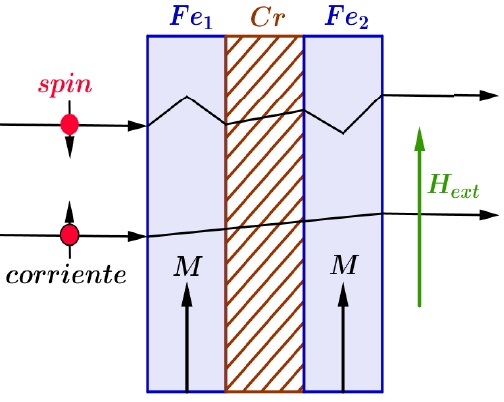
\includegraphics[width=1.0\textwidth]{./Figures/fig337}
	\label{fig:337}
	  \vspace{2.5cm}
  \end{minipage}
\end{figure}

A los diagramas anteriores se puede agregar dos circuitos de la figura \ref{fig:338} que lo complementan indicando $R$ la de mayor resistencia y con r la de menor. Donde los vectores en $R_{\uparrow\uparrow}$ indican igual sentido de la magnetización.

\begin{figure}[H]
    \centering
    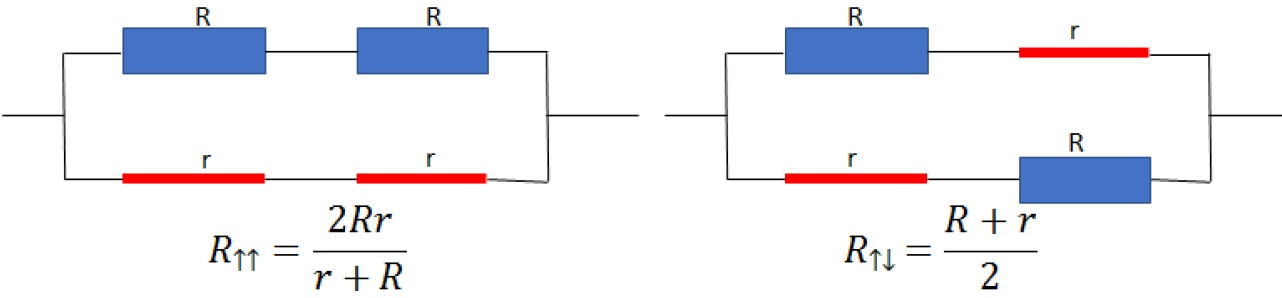
\includegraphics[width=1.0\textwidth]{./Figures/fig338}
	\caption{Válvula de espín}
	\label{fig:338}
\end{figure}

\begin{figure}[H]
  \begin{minipage}[b]{0.47\textwidth}
El siguiente esquema muestra la variación de la resistencia según el campo externo. Esta variación de la impedancia es grande comparada con la hallada por L. Kelvin y es lo que llamamos válvulas de espín. Este hallazgo produjo inmediatamente aplicaciones en los cabezales de lectura de discos duros. Posteriormente hace su aparición un fenómeno más poderoso basado en el efecto túnel.
  \vspace{0cm}
  \end{minipage}
  \hfill
  \begin{minipage}[b]{0.47\textwidth}
     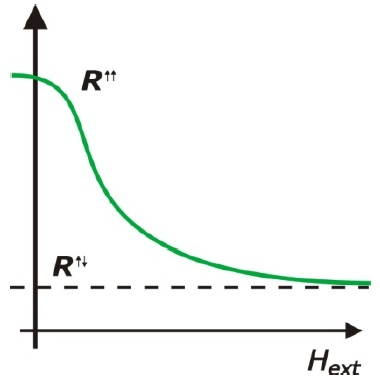
\includegraphics[width=0.8\textwidth]{./Figures/fig339}
	\label{fig:339}
	  \vspace{0cm}
  \end{minipage}
\end{figure}


\subsection{MR de efecto túnel I}

Parecería que la forma más simple de acceder a la Magnetoresistencia de efecto túnel es por medio de los \textbf{ferromagnéticos multicapas} que veremos posteriormente, o bien, como acabamos de ver, por las válvulas de espín

\begin{figure}[H]
  \begin{minipage}[b]{0.47\textwidth}
El sistema para desarrollar la magnetoresistencia de efecto túnel es similar al
descripto para la válvula de spin, salvo que la zona intermedia entre los dos ferromagnéticos es reemplazada por un aislante no magnético. En el 2001 se encontró que usando hierro como material ferromagnético y $MgO$ como aislante, se podría
producir grandes variaciones en la resistencia. Es conveniente, antes de seguir, aclarar el significado del efecto túnel. Es un fenómeno cuántico por el cual una partícula atómica viola un principio de la mecánica clásica y atraviesa una barrera de potencial mayor que la energía cinética de la partícula.

  \vspace{0cm}
  \end{minipage}
  \hfill
  \begin{minipage}[b]{0.47\textwidth}
     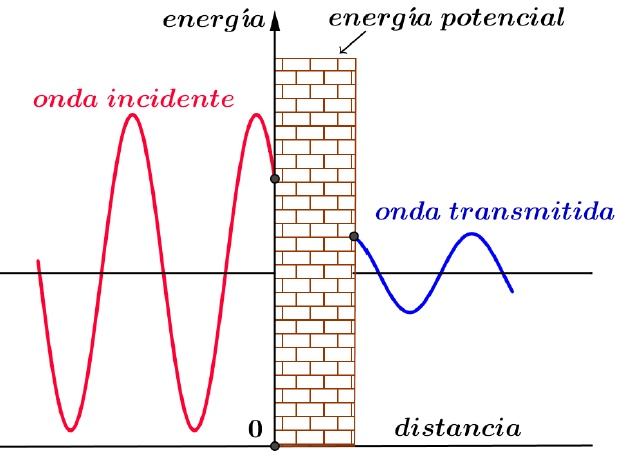
\includegraphics[width=1.0\textwidth]{./Figures/fig340}
	\label{fig:340}
	  \vspace{2cm}
  \end{minipage}
\end{figure}

Las primeras aplicaciones de este fenómeno fueron realizadas en física nuclear, pero luego se extendió a otras áreas que se rigen cuánticamente como, cosmología, semiconductores, microscopio, etc. En el esquema se ejemplifica el fenómeno, no está representada parte de la onda incidente que es refleja. La barrera, representada por la pared, al ser delgada permite que la onda la atraviese y emerja en la capa de la derecha para continuar propagándose. Otra propiedad importante del efecto túnel es que el electrón conserva su orientación durante una determinada distancia de viaje llamada, “longitud de difusión del espín, $\lambda_{sd}$ .Pasada esta distancia el electrón sufre dispersión y olvida la orientación que tenia. Las distancias típica están comprendidas entre $1nm$ hasta $1\mu m$ dependiendo del camino libre medio. Continuaremos con Magnetorresistencia Túnel, pero antes debemos presentar algunosde temas vinculados que ayudarán a su comprensión, estos son: Bandas de Conducción, Aisladores semiconductores y conductores y Electrones libres en un campo magnético.

\subsection{Bandas de conducción}
Con anterioridad comentamos, (ver paramagnetismo de Pauli) la estadística que siguen los electrones cuando se encuentran libres, formando lo que se conoce como un gas de electrones. Las partículas con espín cero y con espín entero se denominan bosones (por el físico Bose) y la de espín semientero fermiones (por Fermi). Siempre a cualquier temperatura los electrones de un metal pueden ser considerados como un gas de electrones, siguiendo la estadística de Fermi. Esta idealización tan simple permite no pensar en los iones del metal, que retienen a los electrones, sino considerar a los electrones que se encuentran en un metal como si estuvieran en un cajón. Pese a su simplicidad en muchos casos se encuentra una buena coincidencia con la realidad.

Veamos cómo se llega a las bandas de conducción en los sólidos y atreves de ellos
explicar la conducción térmica, eléctrica. Para ello retomemos el modelo de los orbitales moleculares y en particular en el metal $Li$ que tiene $Z=3$ luego, la configuración electrónica será $1s^{2}2s^{1}$, por tanto el orbital molecular
para dos átomos será el indicado en la figura \ref{fig:341}

\begin{figure}[H]
    \centering
    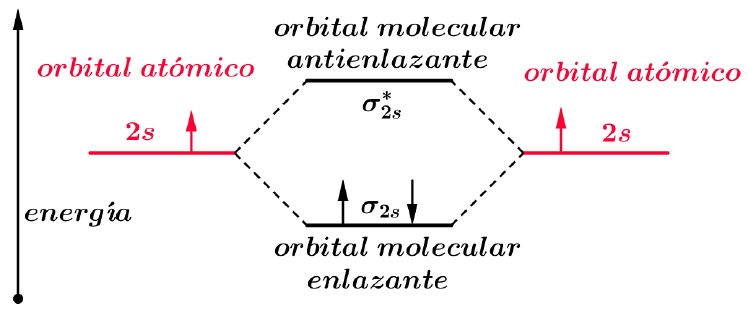
\includegraphics[width=0.6\textwidth]{./Figures/fig341}
	\caption{$Li_{2}$}
	\label{fig:341}
\end{figure}

Para poder generalizar la idea a un sólido se lo representa, como en la figura \ref{fig:342}:

\begin{figure}[H]
    \centering
    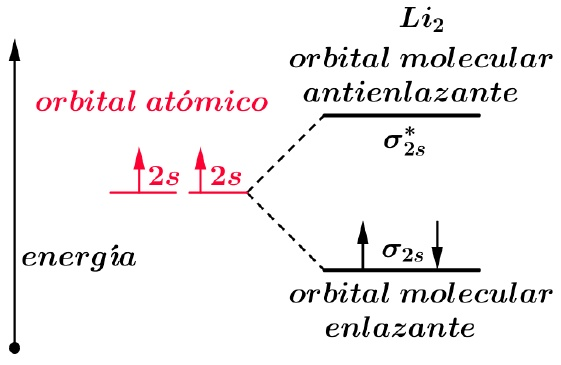
\includegraphics[width=0.4\textwidth]{./Figures/fig342}
	\caption{$Metal_{2}$}
	\label{fig:342}
\end{figure}


Vemos que al ir aumentando la cantidad de átomos crece el número de niveles hasta llegar a un continuo. En algunos metales se solapan ambas bandas. Es simple comprender que con un aumento de temperatura algunos electrones fácilmente pasan a la banda de conducción (ver figura \ref{fig:343}). Al aumentar el número de átomos que interaccionan, aumenta la diferencia de energía entre el orbital molecular más enlazante y el más antienlazante. La mitad de los orbital molecular son esencialmente enlazantes y la otra mitad son antienlazantes. Vemos que al aumentar la cantidad de átomos en el sólido, crece el número de niveles hasta llegar a un continuo. En algunos metales se solapan ambas bandas. Es simple comprender que con un aumento de temperatura algunos electrones fácilmente pasan a la banda de conducción. Banda de valencia es la ocupada por los electrones de mayor energía, mientras que la banda de conducción tiene niveles vacíos de menor energía.

\begin{figure}[H]
    \centering
    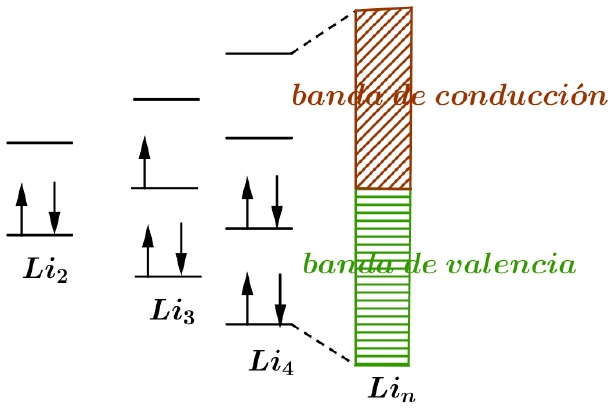
\includegraphics[width=0.6\textwidth]{./Figures/fig343}
	\caption{Bandas de valencia y de conducción}
	\label{fig:343}
\end{figure}

La energía de Fermi $E_{F}$ es la máxima energía ocupada por un electrón a $0^{o}K$, esta energía es importante para el comportamiento de electrones. Los electrones son partículas con espín semientero que verifican el principio de Pauli luego, dos electrones no pueden ocupar simultáneamente el mismo estado cuántico. De esta manera, cuando un sistema posee varios electrones, estos ocuparán niveles de energía mayores a medida que los niveles se llenan, de esta forma se llenan las capas.

En la banda de conducción a $0^{o}K$, no hay electrones aunque hay muchos estados
disponibles. A altas temperaturas, pueden estar pobladas.

Si se combinan $n$ orbitales atómicos para formar un sólido metálico se forman $n$ orbitales moleculares. Si $n$ es grande, la separación de los niveles es pequeña, de manera que tenemos un continuo de niveles y la diferencia de energía entre niveles es pequeña. En este caso los electrones se pueden excitar fácilmente y pasar de un nivel lleno a los vacíos inmediatos, explicando de esta manera la conductividad eléctrica y
térmica.

La importante cantidad de niveles en la banda permite la absorción de radiación de cualquier longitud de onda y también su emisión, explicación su alta reflectividad y también su alta conductividad térmica.

Para que un electrón sea libre debe ser promovido a uno de los estados de energía vacíos de la banda de conducción. Un conductor, necesita muy poca energía para que sus electrones accedan a la banda de conducción, basta una pequeña diferencia de potencial. Por el contrario los aisladores no tienen unidas las capas de valencia y conducción con lo cual resulta complejo que los electrones accedan a la banda de
conducción.

El carbono $C$ (en su forma de diamante) es un aislante eléctrico, la banda de valencia está completamente llena y la banda de conducción está muy alejada como para que los electrones accedan por excitación térmica. El $Si$ y el $Ge$ tienen una diferencia menor entre ambas bandas, por eso son semiconductores. Compuestos como $TiO_{2}$ o $Cd\,S_{2}$ tienen un salto entre bandas pequeño de tal manera que iluminándolos se convierten en conductores.

\subsection{Conductores, semiconductores y aisladores}

Las propiedades eléctricas de los sólidos dependen directa de la estructura de bandas en, véase la figura \ref{fig:344}

\begin{itemize}
	\item[1] El litio tiene la banda de conducción parcialmente ocupada, luego es un conductor.
	
	\item[2] El berilio tiene ocupada totalmente la banda de conducción y solapa con la banda de conducción, es conductor.
	
	\item[3] Si entre la banda de valencia y la de conducción hay una diferencia de
energía de aproximadamente $1eV$, los electrones pueden saltar a la banda de conducción cuando de alguna manera adquieren esa energía. Estamos en presencia de un semiconductor.

	\item[4] Si la energía para acceder a la banda de conducción es elevada y la banda de valencia está llena, estamos en presencia de un aislador.

\end{itemize}


\begin{figure}[H]
    \centering
    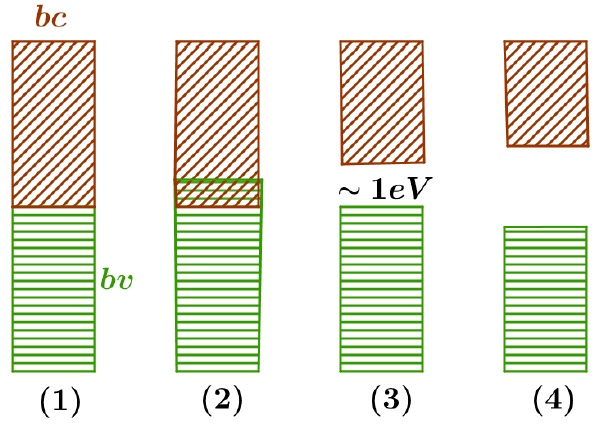
\includegraphics[width=0.5\textwidth]{./Figures/fig344}
	\caption{Conductores, semiconductores y aisladores}
	\label{fig:34}
\end{figure}

Obsérvese en la figura \ref{fig:344} los distintos casos. La conductividad depende de la separación de las bandas. 

Con respecto a la conductividad es frecuente en fase solida. En algunos líquidos la mezcla de orbitales les confiere conducción eléctrica, caso mercurio. En fase gaseosa el comportamiento metálico deja de existir.

La cantidad de energía disponible como resultado de elevar la temperatura del solido es del orden de $kT=0,026\, eV$ a $300^{o}K$, que resulta pequeña si la comparamos con la energía de Fermi que es $7eV$ para el cobre. Esto quiere decir que la energía térmica solo puede interactuar con pocos electrones, ya que la mayoría de los electrones están alejados de la energía de Fermi. Sin embargo estos pocos electrones
dan lugar a fenómenos como la aparición de gradientes de potencial al calentarse a diferente temperaturas los extremos de un conductor dando lugar al efecto Seebeck; complementarios de este último son los efectos Peltier y Thomson.

\subsection{Electrones libres en un campo magnético}

Como fue visto cuando se presento el paramagnetismo de Pauli, los electrones posee una pequeña susceptibilidad paramagnética de volumen.

\begin{figure}[H]
  \begin{minipage}[b]{0.47\textwidth}
En el esquema se muestra la distribución de electrones. el comportamiento de los electrones libres tiene consecuencias cuando sobre dicho material se aplica un campo magnético $H$ externo. Si un espín se alineado con el campo externo tienen menos energía que los antialineados y la energía conjunta de todos los electrones ser aproximadamente la $E_{F}$.
  \vspace{0cm}
  \end{minipage}
  \hfill
  \begin{minipage}[b]{0.47\textwidth}
     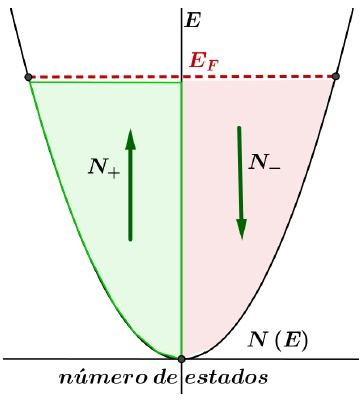
\includegraphics[width=0.9\textwidth]{./Figures/fig345}
	\label{fig:345}
	  \vspace{0cm}
  \end{minipage}
\end{figure}


\begin{figure}[H]
  \begin{minipage}[b]{0.47\textwidth}
Luego, en un metal, mantener esa energía constante implica que algunos electrones anti-alineados deben alinearse con el campo $H$. Sin campo las poblaciones de espines alineados y anti-alineados es más o menos la misma, pero en presencia de campo debe aumentar el número de alineados y decrecer el número de desalineados, superando el número de momentos magnéticos alineados a los antialineados. Esto ya fue comentado.
  \vspace{0cm}
  \end{minipage}
  \hfill
  \begin{minipage}[b]{0.47\textwidth}
     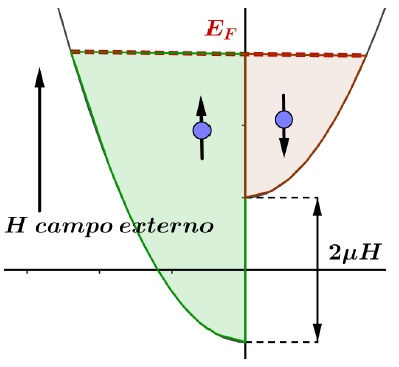
\includegraphics[width=0.9\textwidth]{./Figures/fig346}
	\label{fig:346}
	  \vspace{0.5cm}
  \end{minipage}
\end{figure}

\subsection{MR de efecto túnel II}

Los electrones viajan a la sub-banda que presentan la misma orientación de espín, ya que conservan la orientación durante el efecto túnel. Esto es efectivo cuando se aplica un voltaje y los electrones viajan de izquierda a derecha , dependiendo de la disponibilidad de estados libres. Por tanto si $Fe_{1}$ y $Fe_{2}$ poseen la misma orientación de sus momentos magnéticos (caso de la izquierda) los electrones encontraran los mismos estados de orientación en el otro, ocasionando una importante corriente túnel (véase la figura \ref{fig:347}).

\begin{figure}[H]
    \centering
    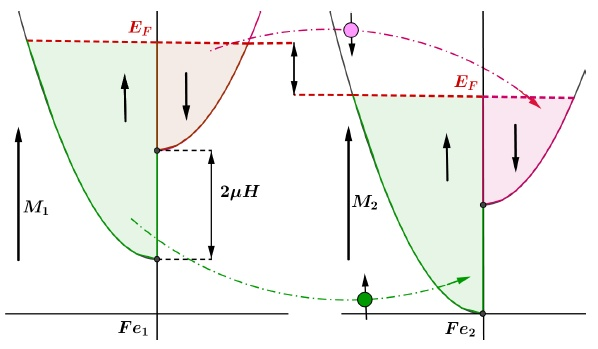
\includegraphics[width=0.7\textwidth]{./Figures/fig347}
	\caption{Efecto túnel On}
	\label{fig:347}
\end{figure}


Pero, si los momentos magnéticos son antiparalelos ambas direcciones tendrán dificultades, siendo la corriente túnel pequeña (véase la figura \ref{fig:348}). 

\begin{figure}[H]
    \centering
    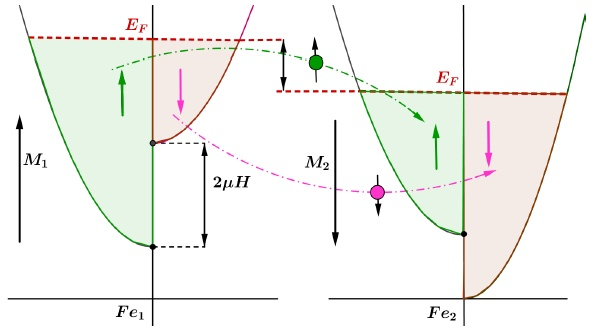
\includegraphics[width=0.7\textwidth]{./Figures/fig348}
	\caption{Efecto túnel Off}
	\label{fig:348}
\end{figure}

Dicho de otro modo: La corriente que pasa a través del efecto túnel, por el aislador que conecta los dos ferromagnéticos, depende de la dirección de la magnetización. Si la magnetización de los dos ferromagnéticos es paralela entre sí, entonces la corriente del túnel es alta. Luego, una alineación antiparalela de magnetización de los dos ferromagnéticos disminuye el flujo de corriente. Esta magnetización es comandada por un campo externo $H$.

\begin{figure}[H]
  \begin{minipage}[b]{0.47\textwidth}
luego hacemos pasar una corriente perpendicular a las capas mencionadas. Los electrones al pasar por la primera placa gruesa, (generalmente llamada "capa fija") se polarizaran según $M_{1}$, entonces en la segunda placa tenemos una corriente polarizada de espín. Esta corriente de espín polarizada accede a la tercera placa ferromagnética, más delgada (la "capa libre"), el momento angular puede transferirse a esta capa, cambiando su orientación, normalmente habrá un cierto ángulo entre la polarización de los espines y la magnetización local $M_{2}$. Si esta suposición es correcta los electrones precesan. Los efectos generalmente solo se ven en dispositivos a escala nanométrica.
  \vspace{0cm}
  \end{minipage}
  \hfill
  \begin{minipage}[b]{0.47\textwidth}
     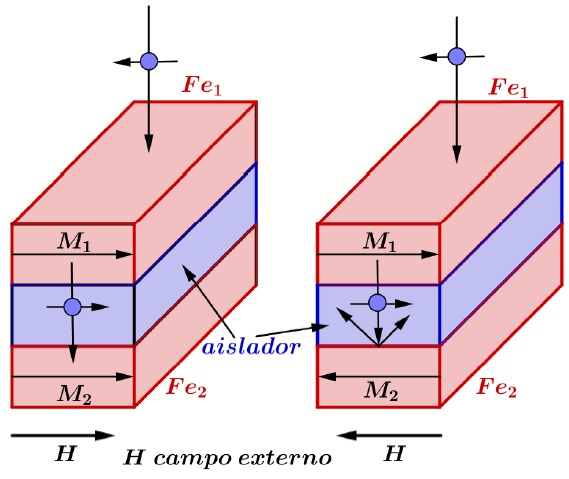
\includegraphics[width=1.0\textwidth]{./Figures/fig349}
	\label{fig:349}
	  \vspace{1.5cm}
  \end{minipage}
\end{figure}


\subsection{Consecuencias de la transferencia de espín}

Los estados magnéticos de un sólido son controlados y manipulados clásicamente a través de campos magnéticos aplicados. En 1996 J.C. Slonczewski y l. Berger, predijeron teóricamente el fenómeno de la transferencia de torque de espín. La transferencia de torque por el espín es un efecto en el cual la orientación de una capa magnética en una unión de túnel magnético o válvula de spin puede modificarse usando una corriente de spin polarizada. Vimos que una corriente eléctrica generalmente no está polarizada, consiste en un \textbf{50\%} de spin-up y un \textbf{50\%} de spin-down. una corriente polarizada tiene mayormente los electrones en una sola dirección. Al pasar una corriente (no polarizada) a través de una capa magnética gruesa (en espesor, generalmente llamada "capa fija"), se produce una corriente polarizada. Si esta corriente se dirige a una segunda capa magnética más delgada (“capa libre"), el momento angular se transfiere a esta capa, cambiando la orientación magnética. Esto puede usarse para excitar oscilaciones o incluso cambiar la orientación del imán. Los efectos generalmente solo se ven en dispositivos a escala nanométrica. Para describirlo consideramos el esquema formado por dos capas de material ferromagnético separados por un conductor no magnético como en el caso de válvula de espín.

Como fue comentado, son dos las posibles acciones de la corriente de espín:

\begin{itemize}
	\item[1] Una importante corriente puede, en principio, generar un torque lo suficientemente grande como para cambiar la dirección de magnetización del material que está atravesando.
	 
	\item[2] La teoría muestra que, en ciertas situaciones, el par de transferencia de spin puede provocar que la magnetización de una capa ferromagnética gire alrededor, en precesión, a una frecuencia controlada por la corriente. Esta técnica hace posible los osciladores en el orden de los gigahercios con una amplia gama de usos electrónicos.

\end{itemize}

Considere el esquema de la figura \ref{fig:350} donde la capa fija tiene su magnetización $M_{1}$ permanente y la capa libre tiene una dirección de magnetización arbitraria $M_{2}$. Una corriente eléctrica no polarizada que pasa de izquierda a derecha se polarizaría después de pasar por capa libre. A medida que se inyectan en la capa libre, los espines de electrones se realinean hacia la dirección de $M_{2}$. Sin embargo, debido a la conservación del momento angular, el impulso de los spin también se transfiere a $M_{2}$. Por lo tanto, la magnetización $M_{2}$ siente un par con la misma dirección de $M_{1}$.

\begin{figure}[H]
    \centering
    \includegraphics[width=0.8\textwidth]{./Figures/fig350}
	\caption{Realineación de espines}
	\label{fig:350}
\end{figure}


\subsection{Estados magnéticos del sólido}

Los estados magnéticos de un sólido son controlados y manipulados clásicamente a través de campos magnéticos aplicados. En 1996 J.C. Slonczewski y l. Berger, predijeron teóricamente el fenómeno de la transferencia de torque de espín. La transferencia de torque por el espín es un efecto en el cual la orientación de una capa magnética en una unión de túnel magnético o válvula de spin puede modificarse usando una corriente de spin polarizada. Vimos que una corriente eléctrica generalmente no está polarizada, consiste en un 50\% de spin-up y un 50\% de spin-down. una corriente polarizada tiene mayormente los electrones en una sola dirección. Al pasar una corriente (no polarizada) a través de una capa magnética gruesa (en espesor, generalmente llamada "capa fija"), se produce una corriente polarizada. Si esta corriente se dirige a una segunda capa magnética más delgada (“capa libre"), el momento angular se transfiere a esta capa, cambiando la orientación magnética. Esto puede usarse para excitar oscilaciones o incluso cambiar la orientación del imán. Los efectos generalmente solo se ven en dispositivos a escala nanométrica. Para describirlo consideramos el esquema formado por dos capas de material ferromagnético separados por un conductor no magnético como en el caso de válvula de espín.

Como fue comentado, son dos las posibles acciones de la corriente de spin:

\begin{itemize}
	\item[1] Una importante corriente puede, en principio, generar un torque lo suficientemente grande como para cambiar la dirección de magnetización del material que está atravesando.
	
	\item[2] la teoría muestra que, en ciertas situaciones, el par de transferencia de espín puede provocar que la magnetización de una capa ferromagnética gire alrededor, en precesión, a una frecuencia controlada por la corriente. Esta técnica hace posible los osciladores en el orden de los gigahercios con una amplia gama de usos electrónicos.
	
\end{itemize}

\textbf{Repetimos con otras palabras lo antes dicho:}


\subsection{Filtro de espín}

Un material ferromagnético actúa como un filtro de espín absorbiendo las componentes transversales del momento del spin y dejando una corriente polarizada. Cuando esta corriente se inyecta en otro material ferromagnético se produce el mismo efecto de filtrado de espín. Los componentes de la polarización del espín transversal a la magnetización del segundo ferromagnético se absorben y aplican un par a la magnetización que es el par de transferencia de spin. Por lo tanto, la corriente de espín polarizada aplicaría un par a la magnetización del segundo ferromagnético si la corriente de polarización y la magnetización no son colineales. Ver esquema. Tenga en cuenta que el efecto de transferencia de torque también está presente cuando los electrones pasar a través de la capa fija. sin embargo, dado que capa fija es de mayor tamaño, el efecto es insignificante.

\begin{figure}[H]
    \centering
    \includegraphics[width=0.5\textwidth]{./Figures/fig41}
	\caption{Transferencia del momento}
	\label{fig:41}
\end{figure}

